\documentclass{beamer}
\usepackage{caption}
\usepackage[utf8]{inputenc}
\usepackage[T1]{fontenc}
\usepackage{tikz}
\usepackage{fancyvrb}

% Pour quel partie chaque personne parle :
% Mise en contexte -> Vital
% Technologies utilisées -> Vital
% Différentes stratégies pour un rendu 3D :
%   Approche historique -> Matthieu
%   Explication de DDA  -> Matthieu
%   Approche moderne -> Matthieu
% Construction de mur -> Vital
% Les collisions -> Elian
% Les portails -> Elian
% Les renders -> Matthieu
% Conclusion -> Elian


\usetheme{Boadilla}

\begin{document}

% Définition de la mise en page du pied de page avec un espacement réduit
\setbeamertemplate{footline}{%
  \leavevmode%
  \hbox{\begin{beamercolorbox}[wd=\paperwidth,ht=2.25ex,dp=1ex,center]{author in head/foot}%
    \usebeamerfont{author in head/foot}\insertshortauthor\hspace*{2em}
    \insertshorttitle\hspace*{2em}\insertframenumber{} / \inserttotalframenumber
  \end{beamercolorbox}}%
  \vskip0pt%
}

\title{Présentation du projet Portal 0.0}
\author[BADSTÜBER E. BIDAULT M. FOCHEUX V.]{BADSTÜBER Elian BIDAULT Matthieu FOCHEUX Vital \\
                                                Licence 3 Informatique}
\date{Mars 2024}

\AtBeginSubsection[]
{
  \begin{frame}<beamer>
    \frametitle{Plan}
    \tableofcontents[currentsection,currentsubsection,subsubsectionstyle=show/show/hide/hide]
  \end{frame}
}

\setcounter{framenumber}{0}
% \setbeamertemplate{page number in head/foot}{}

{
\setbeamertemplate{footline}{}
\begin{frame}
    \titlepage
    
    \vfill % Insertion d'un espace vertical flexible pour pousser le texte en bas
    \begin{columns}
        \column{0.3\textwidth}
        \centering
        
\includegraphics[width=\textwidth]{images/logo-UFR-ST.jpg} 
    
        \column{0.4\textwidth}
        \begin{flushright}
            \small Tuteur : Julien BERNARD
        \end{flushright}    
    \end{columns}
\end{frame}
}

\setcounter{framenumber}{0}
\setbeamertemplate{page number in head/foot}[totalframenumber]

\begin{frame}
    \frametitle{Table des matières}
    \tableofcontents
\end{frame}

\section{Introduction}

\begin{frame}
    \frametitle{Introduction \\
                \small Système de jeu}
    \begin{block}{}
        \begin{itemize}
            \item Portal 0.0 $\rightarrow $ principes techniques de plusieurs jeux vidéos connus
        \end{itemize}
    \end{block}
    \begin{block}{}
        \begin{itemize}
            \item Résolution d'énigmes à l'aide de portails
            \item Téléportation lorsqu'on passe à travers
            \item Principe de Portal (2007)
        \end{itemize}
    \end{block}
    \begin{figure}
        \centering
        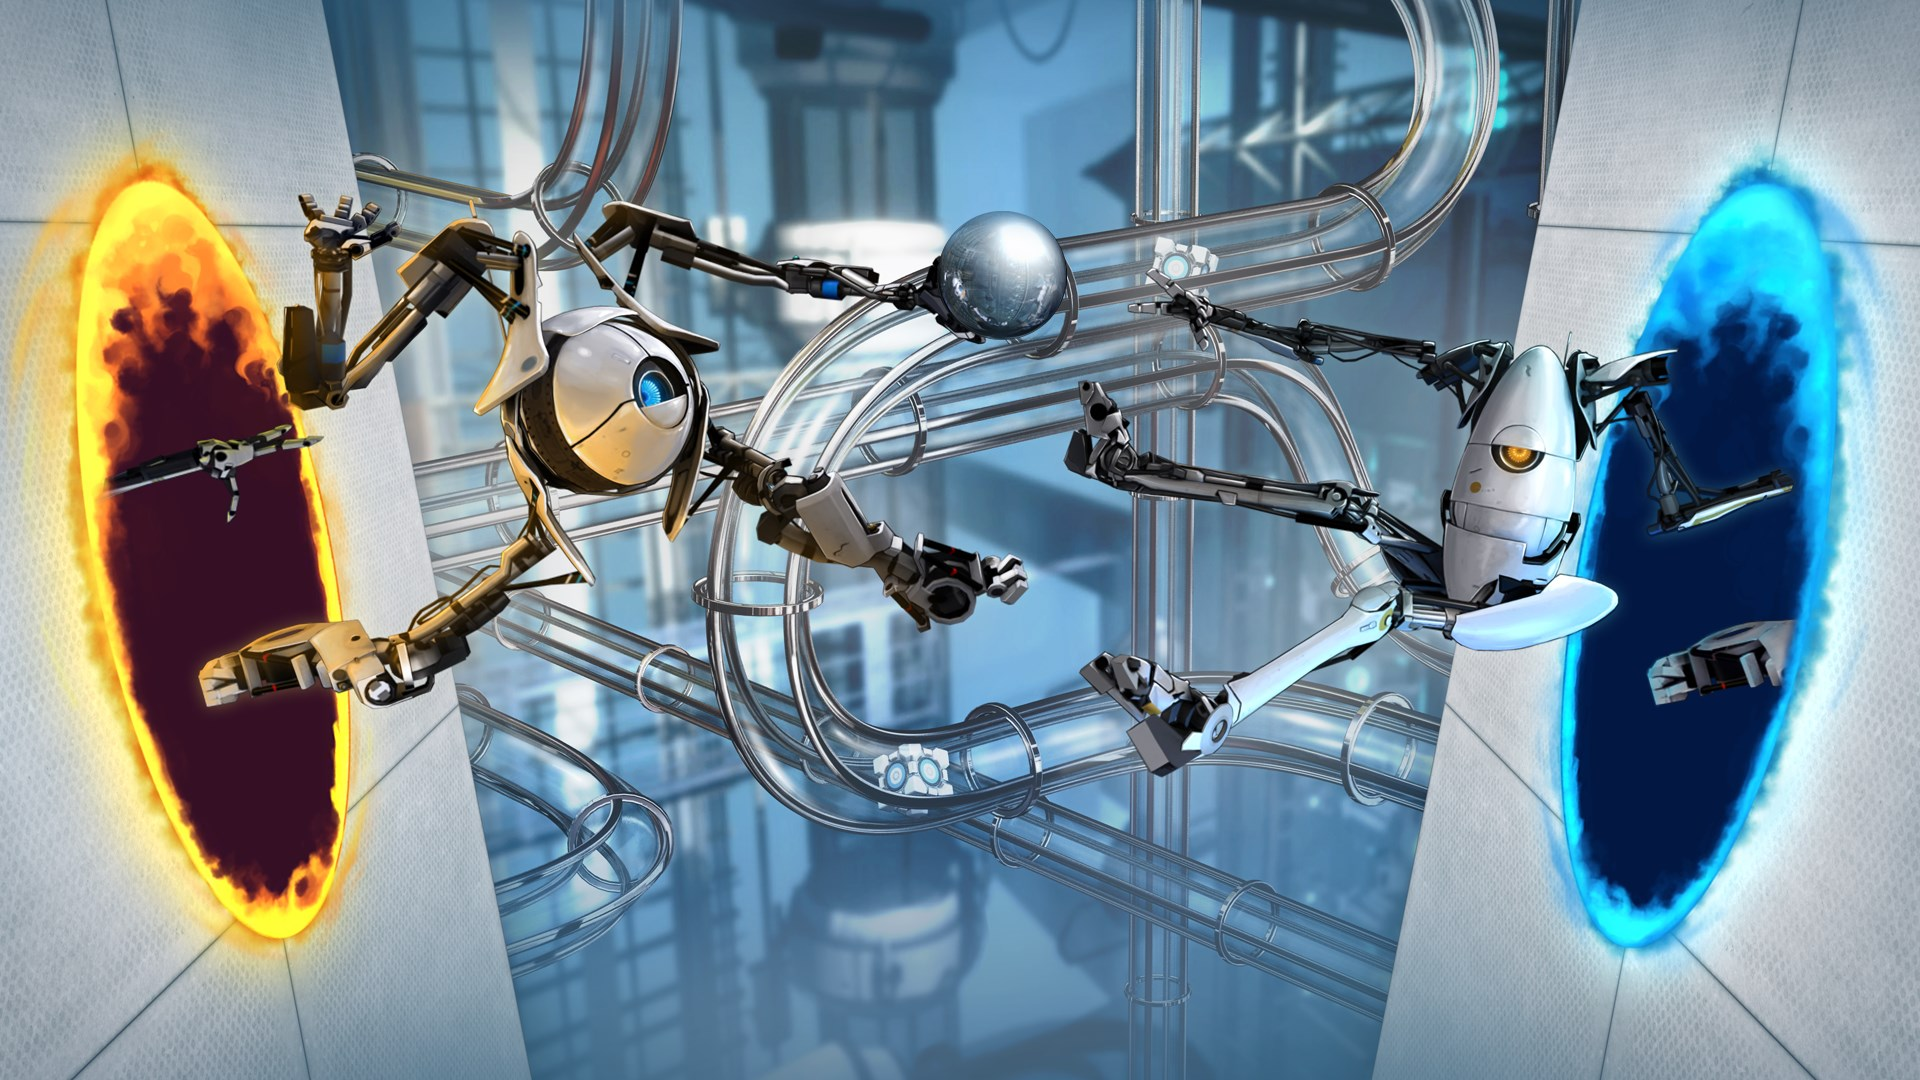
\includegraphics[width=0.5\textwidth]{images/portal.jpg}
        \caption{Portal (2007)}
    \end{figure}
\end{frame}

\begin{frame}
    \frametitle{Introduction \\
                \small Technique graphique}
    \begin{block}{}
        \begin{itemize}
            \item Portal 0.0 $\rightarrow $ principes techniques de plusieurs jeux vidéos connus
        \end{itemize}
    \end{block}
    \begin{block}{}
        \begin{itemize}
            \item Méthode raycasting
            \item Rendu 2.5D popularisé dans les années 90
            \item Principe de Wolfenstein3D (1992)
        \end{itemize}
    \end{block}
    \begin{figure}
        \centering
        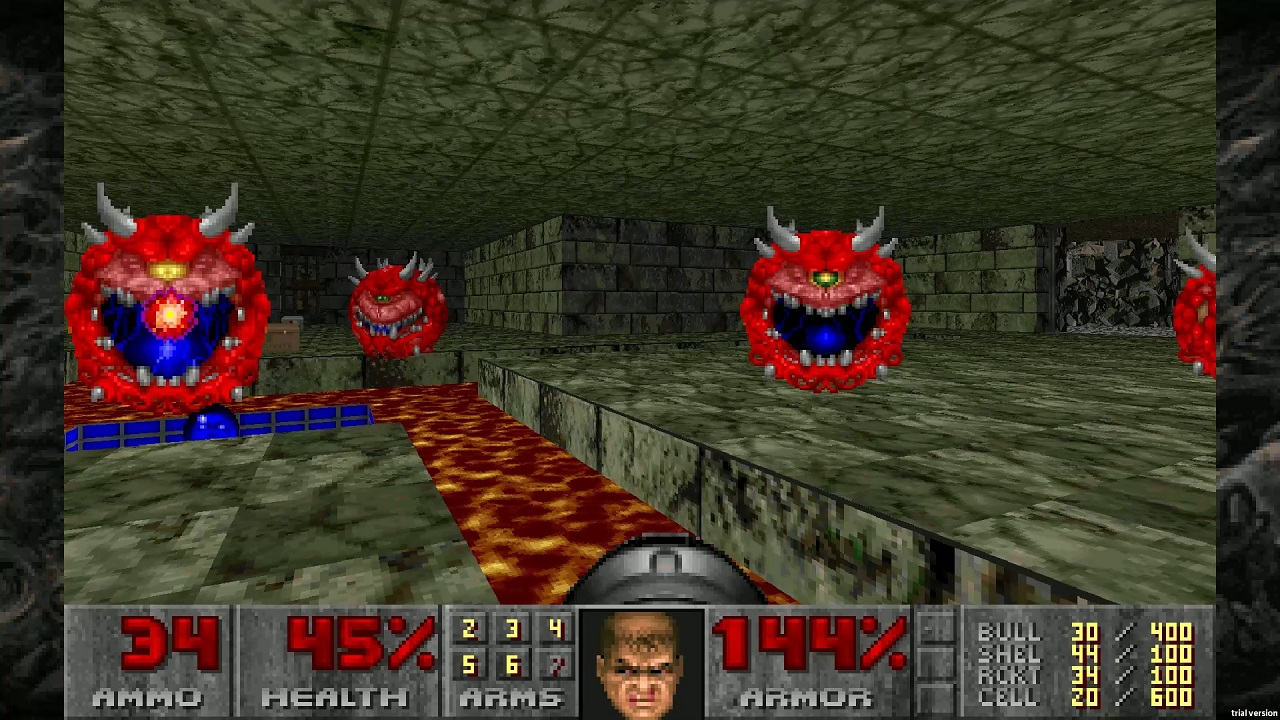
\includegraphics[width=0.5\textwidth]{images/doom_1993.jpg}
        \caption{Doom (1993)}
    \end{figure}
\end{frame}

\begin{frame}
    \frametitle{Introduction \\
                \small Technologies utilisées}
    \hspace{5mm}
    \raisebox{-8mm}{
        
\includegraphics[width=0.25\textwidth]{images/cpp.png}
    }
    \hspace{-1mm}
    \raisebox{-8mm}{
        
\includegraphics[width=0.33\textwidth]{images/GF.png}
    }
    \hspace{-15mm}
    
\includegraphics[width=0.40\textwidth]{images/github.png}
\end{frame}

\section{Algorithmes et techniques}

\subsection{Construction de mur}

\begin{frame}
    \frametitle{Construction de mur \\
                \small Commencement}
    \begin{block}{}
        \begin{itemize}
            \item Création de la carte à partir d'un PNG
            \item Récupération des coordonnées des cellules à l'aide d'un parcours en profondeur
        \end{itemize}
    \end{block}
    \hspace{5mm}
    \begin{minipage}{\textwidth}
        \begin{minipage}{0.25\textwidth}
            \begin{figure}
                
\begin{tikzpicture}[scale=0.3]
            
                    \fill[line width=1pt] (0, 0) -- (0, 10) -- (10, 10) -- (10, 0) -- cycle;
                    \fill[white] (1, 1) -- (6, 1) -- (6, 3) -- (3, 3) -- (3, 4) -- (8, 4) -- (8, 3) -- (7, 3) -- (7, 1) -- (9, 1) -- (9, 7) -- (8, 7) -- (8, 8) -- (9, 8) -- (9, 9) -- (7, 9) -- (7, 6) -- (6, 6) -- (6, 7) -- (4, 7) -- (4, 8) -- (6, 8) -- (6, 9) -- (3, 9) -- (3, 7) -- (2, 7) -- (2, 9) -- (1, 9) -- (1, 6) -- (5, 6) -- (5, 5) -- (1, 5) -- cycle;
                
                
                    \draw[color=lightgray] (2, 5) -- (2, 1);
                    \draw[color=lightgray] (2, 9) -- (2, 6);
                
                    \draw[color=lightgray] (3, 5) -- (3, 1);
                    \draw[color=lightgray] (3, 9) -- (3, 6);
                
                    \draw[color=lightgray] (4, 3) -- (4, 1);
                    \draw[color=lightgray] (4, 5) -- (4, 4);
                    \draw[color=lightgray] (4, 9) -- (4, 6);
                
                    \draw[color=lightgray] (5, 3) -- (5, 1);
                    \draw[color=lightgray] (5, 7) -- (5, 4);
                    \draw[color=lightgray] (5, 9) -- (5, 8);
                
                    \draw[color=lightgray] (6, 7) -- (6, 4);
                    \draw[color=lightgray] (6, 9) -- (6, 8);
                
                    \draw[color=lightgray] (7, 7) -- (7, 4);
                    \draw[color=lightgray] (7, 9) -- (7, 8);
                    \draw[color=lightgray] (8, 9) -- (8, 1);
                
                
                    \draw[color=lightgray] (1, 9) -- (2, 9);
                    \draw[color=lightgray] (3, 9) -- (6, 9);
                    \draw[color=lightgray] (7, 9) -- (9, 9);
                
                    \draw[color=lightgray] (1, 7) -- (6, 7);
                    \draw[color=lightgray] (7, 7) -- (9, 7);
                
                    \draw[color=lightgray] (1, 6) -- (9, 6);
                
                    \draw[color=lightgray] (1, 5) -- (9, 5);
                    
                    \draw[color=lightgray] (1, 4) -- (9, 4);
                
                    \draw[color=lightgray] (1, 3) -- (6, 3); 
                    \draw[color=lightgray] (7, 3) -- (9, 3);
                    
                    \draw[color=lightgray] (1, 2) -- (6, 2); 
                    \draw[color=lightgray] (7, 2) -- (9, 2);
                    
                \end{tikzpicture}
            \end{figure}
        \end{minipage}
        \hspace{5mm}
        \begin{minipage}{0.7\textwidth}
            \begin{block}{}
                \begin{itemize}
                    \item Les coordonnées des cellules corresondent au coin supérieur gauche de chaque cellule
                    \item Une cellule correspond à un bloc unitaire de la carte
                \end{itemize}                
            \end{block}
        \end{minipage}
        
    \end{minipage}
\end{frame}

\begin{frame}
    \frametitle{Construction de mur \\
                \small Sommets utiles}
    \begin{block}{}
        \begin{itemize}
            \item Boucle sur les coordonnées des cellules
            \item Parité du nombre de cellules adjacentes
        \end{itemize}
    \end{block}
    \begin{figure}
        \centering
        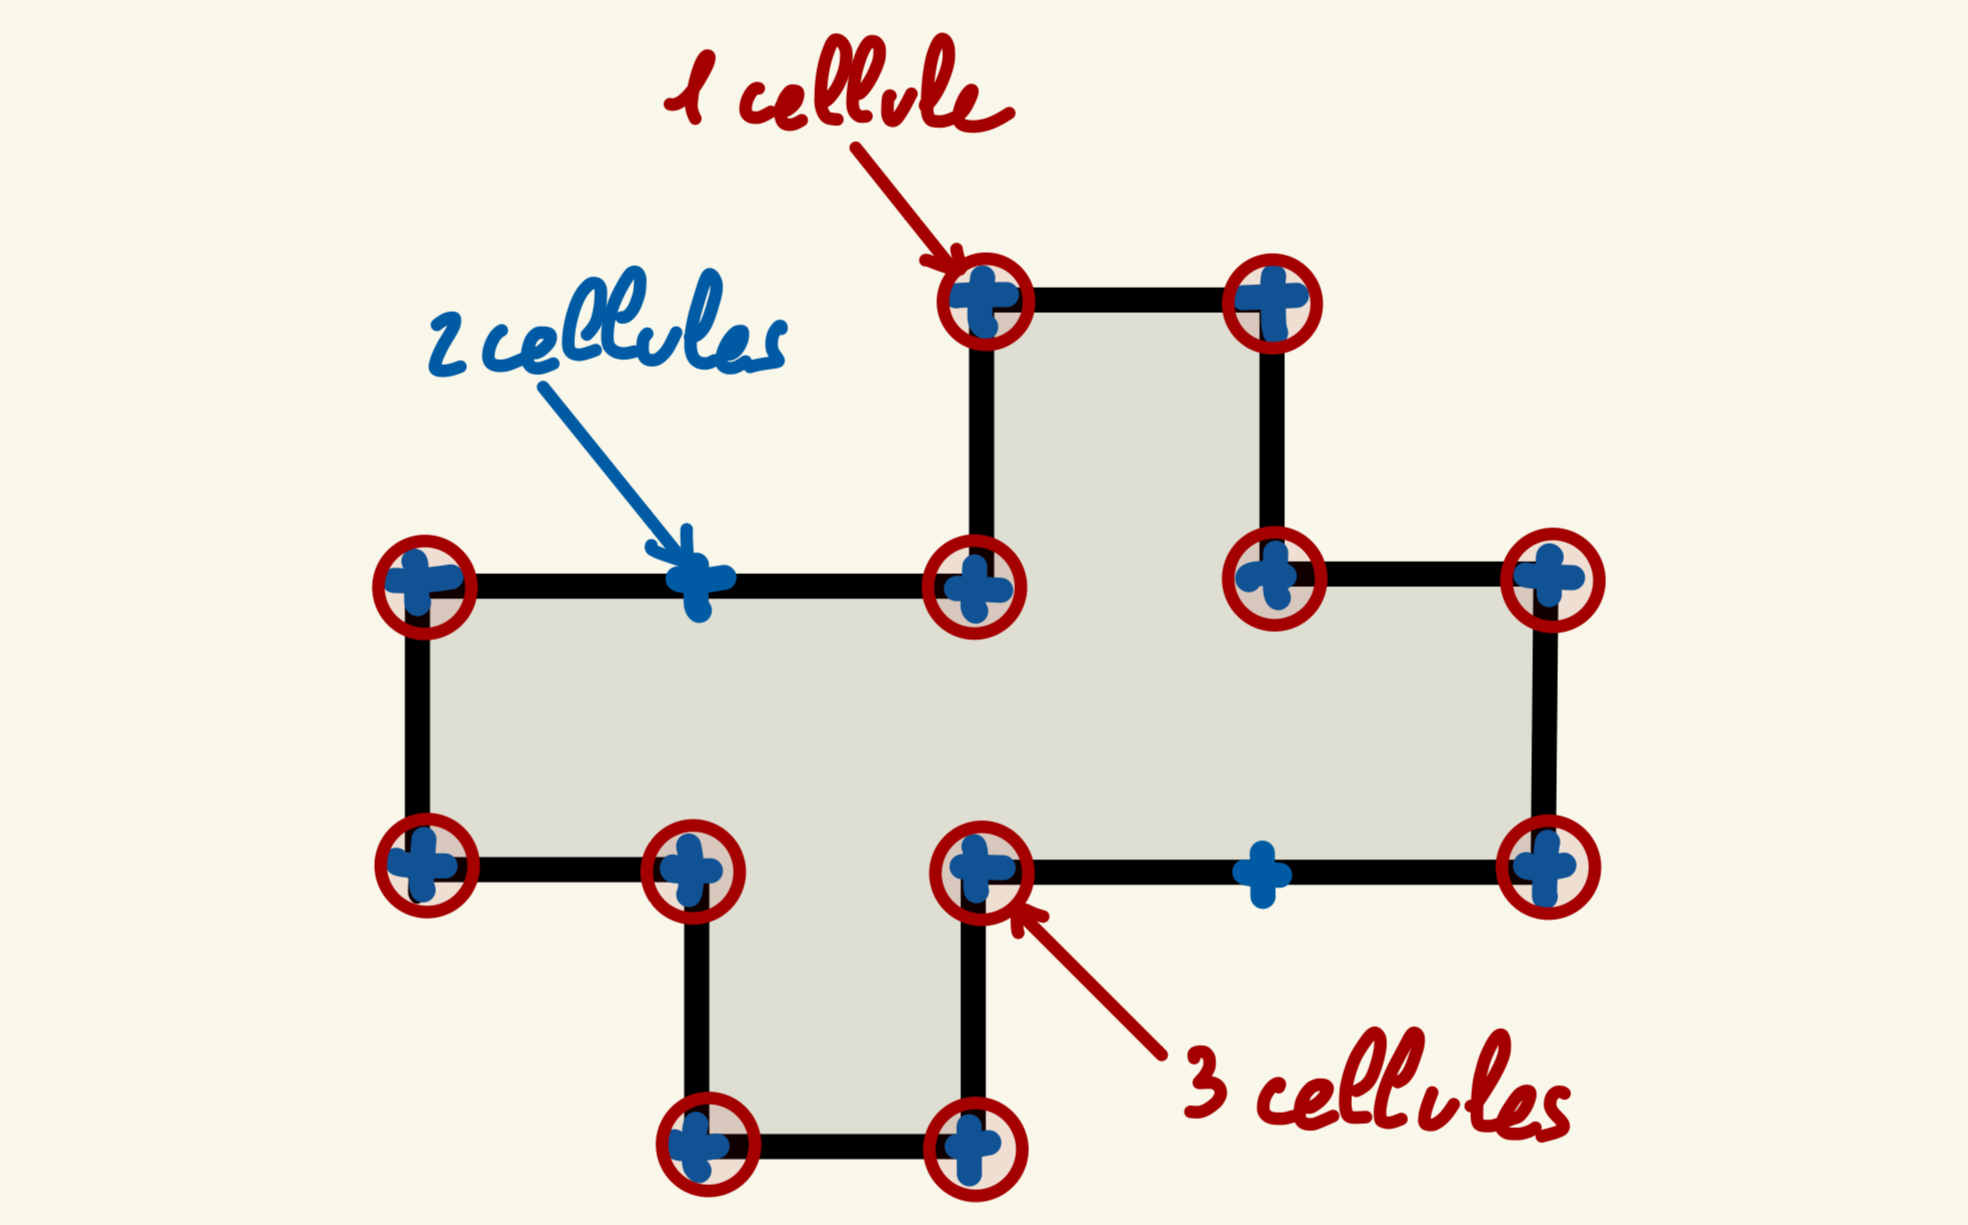
\includegraphics[width=0.7\textwidth]{images/sommets_utiles.jpg}
    \end{figure}
\end{frame}

\begin{frame}[fragile]
    \frametitle{Construction de mur \\
                \small Trie des sommets}
    \hspace*{-2.5cm}
    \begin{minipage}[t][3.5cm][t]{-1\textwidth} % La hauteur est contrôlée ici, ajustez 3cm selon vos besoins
       
        \begin{verbatim}
            d = {'d', 'b', 'g', 'h'}
            dir = d[i%4], dir2 = d[(i+1)%4]
            while(v.contient(sommetA(dir)) ou v.contient(sommetA(dir2))):
                if canGo(dir) and !canGo(dir2):
                    v <- sommetA(dir)
                else:
                    v <- sommetA(dir2)
                    echange(dir, dir2)
        \end{verbatim}
    \end{minipage}
    \begin{figure}
        \centering
        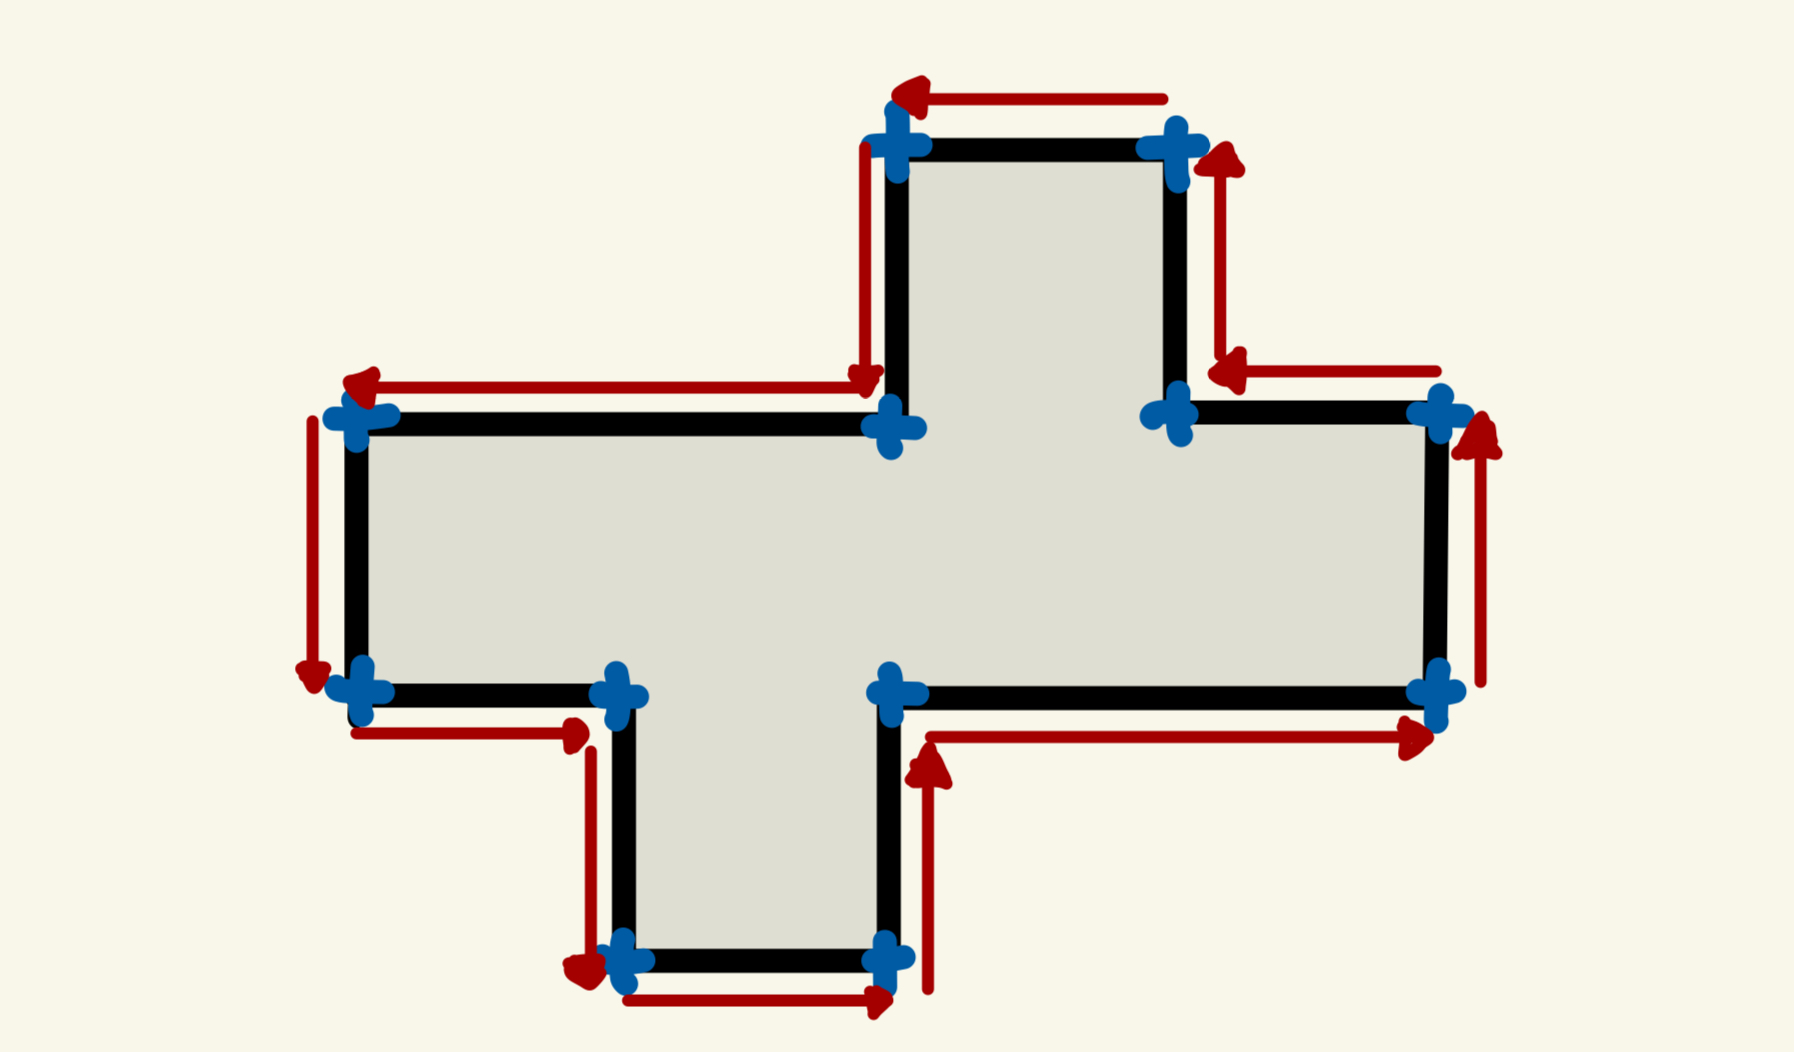
\includegraphics[width=0.5\textwidth]{images/tri_sommet.jpg}
    \end{figure}
\end{frame}

\subsection{Les collisions}

\begin{frame}
    \frametitle{Les collisions \\
                \small Système de collision cercle/rectangle}
    \begin{figure}
        \centering
        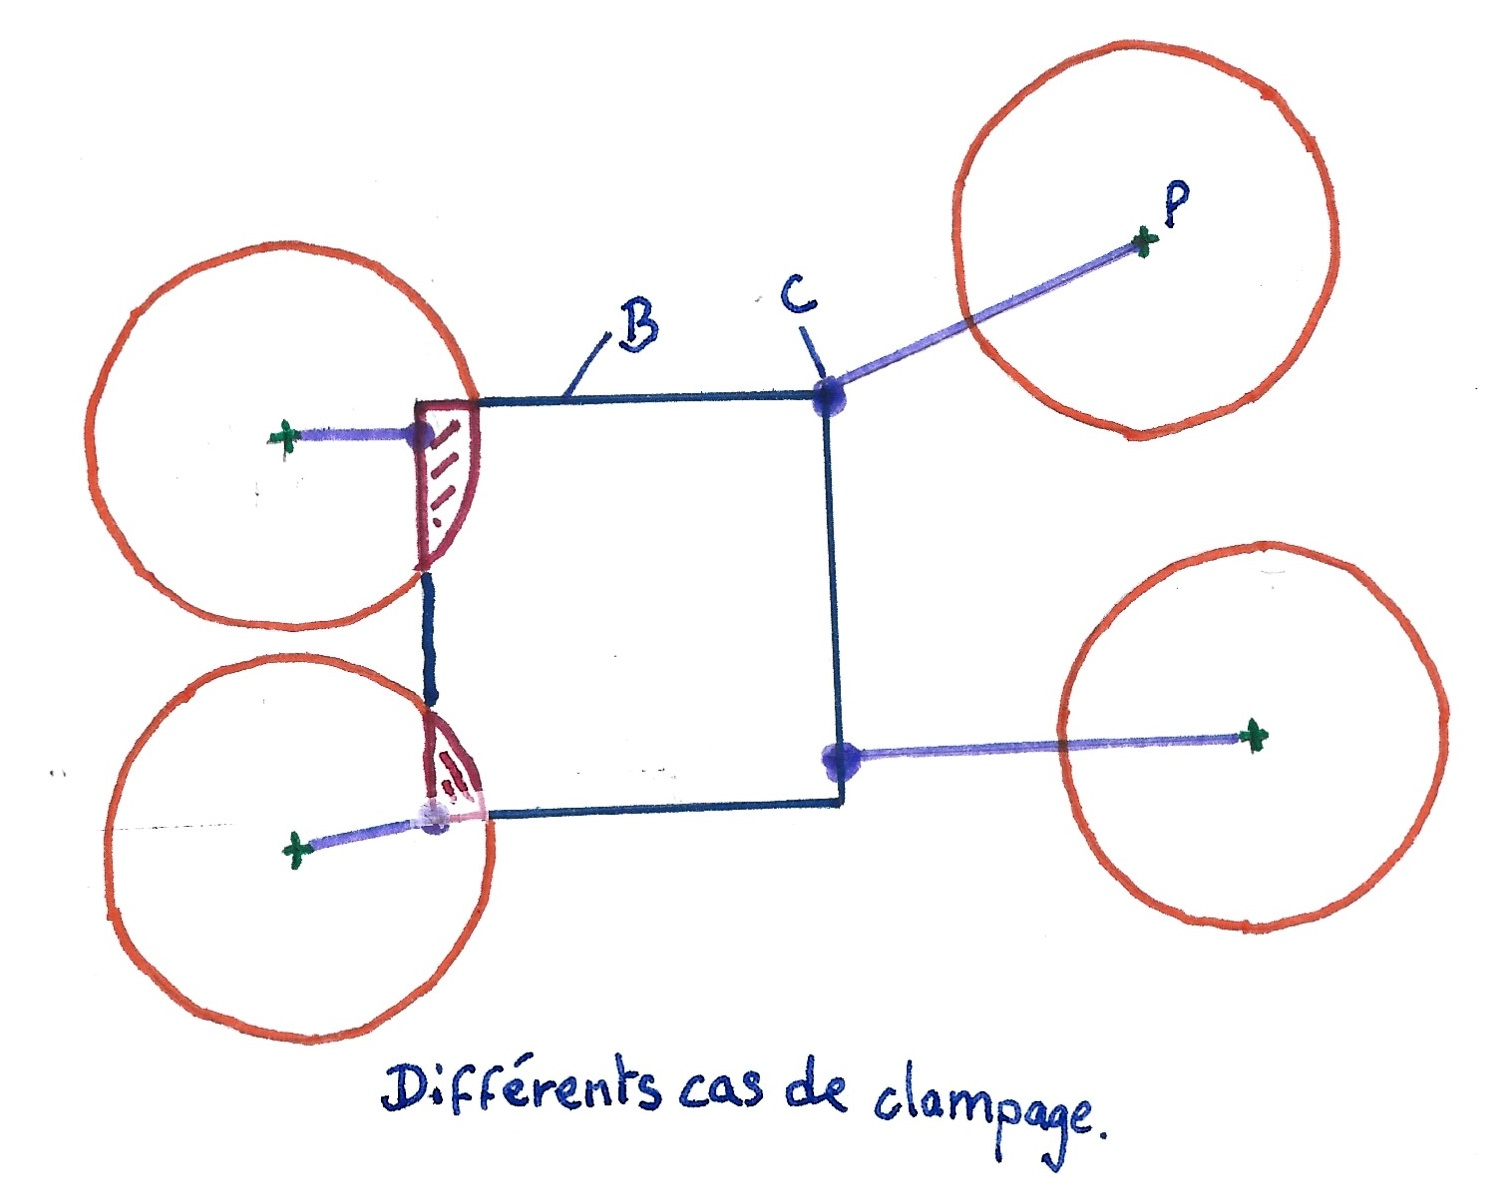
\includegraphics[width=0.4\textwidth]{images/fig4.jpg}
    \end{figure}
    \begin{block}{}
        \begin{itemize}
            \item Recherche du point le plus proche
            \begin{itemize}
                \item méthode de clampage
            \end{itemize}
            \item Validation de proximité
            \begin{itemize}
                \item replacement du personnage en cas de collision
            \end{itemize}
        \end{itemize}
    \end{block}
\end{frame}

\subsection{Différentes stratégies pour un rendu 3D}

\begin{frame}
    \frametitle{Différentes stratégie pour un rendu 3D \\
                \small Approche historique}
    \begin{block}{Raycasting}
        \begin{itemize}
            \item Projection de rayons depuis la position du joueur.
            \item Pour chaque colonnes de pixels de la fenêtre.
        \end{itemize}
    \end{block}

    \begin{figure}
        \center
        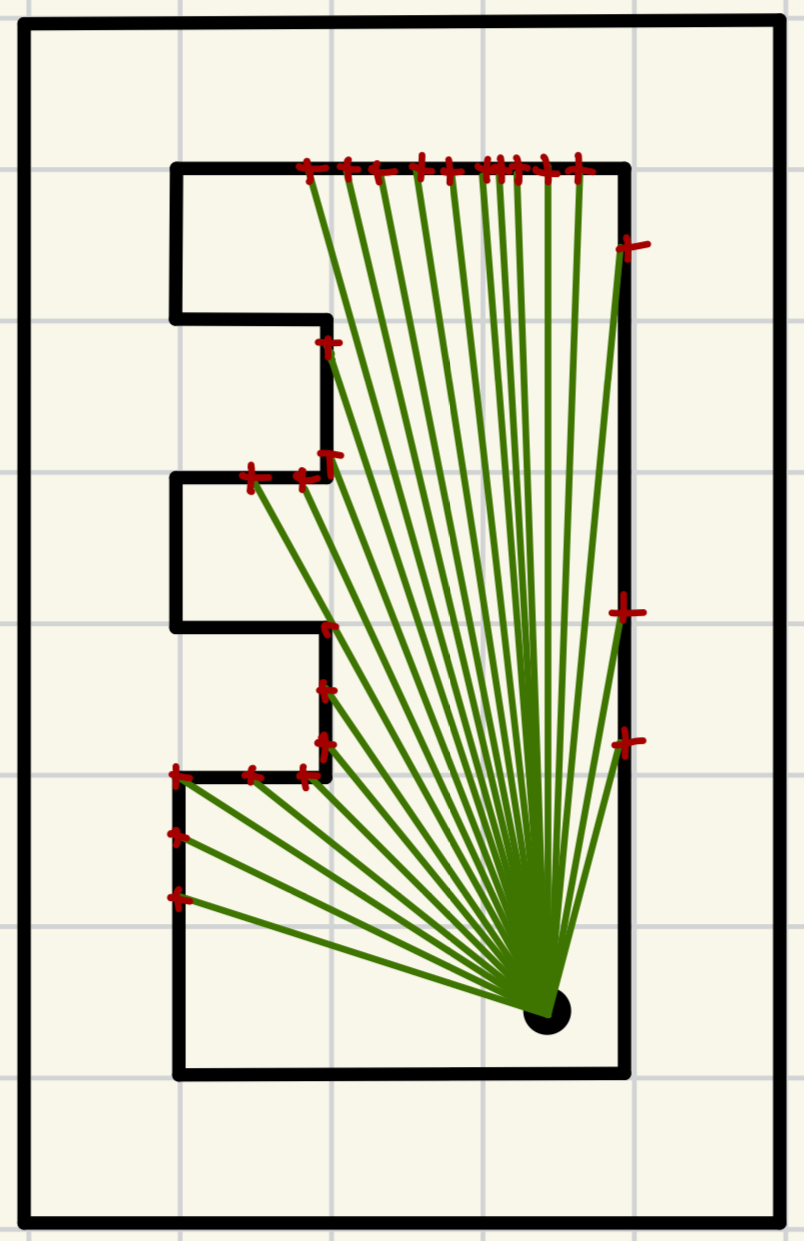
\includegraphics[width=0.25\textwidth]{images/projection2D.jpeg}
        \raisebox{2cm}{
            \hspace{2mm}$\Longrightarrow$\hspace{2mm}
        }
        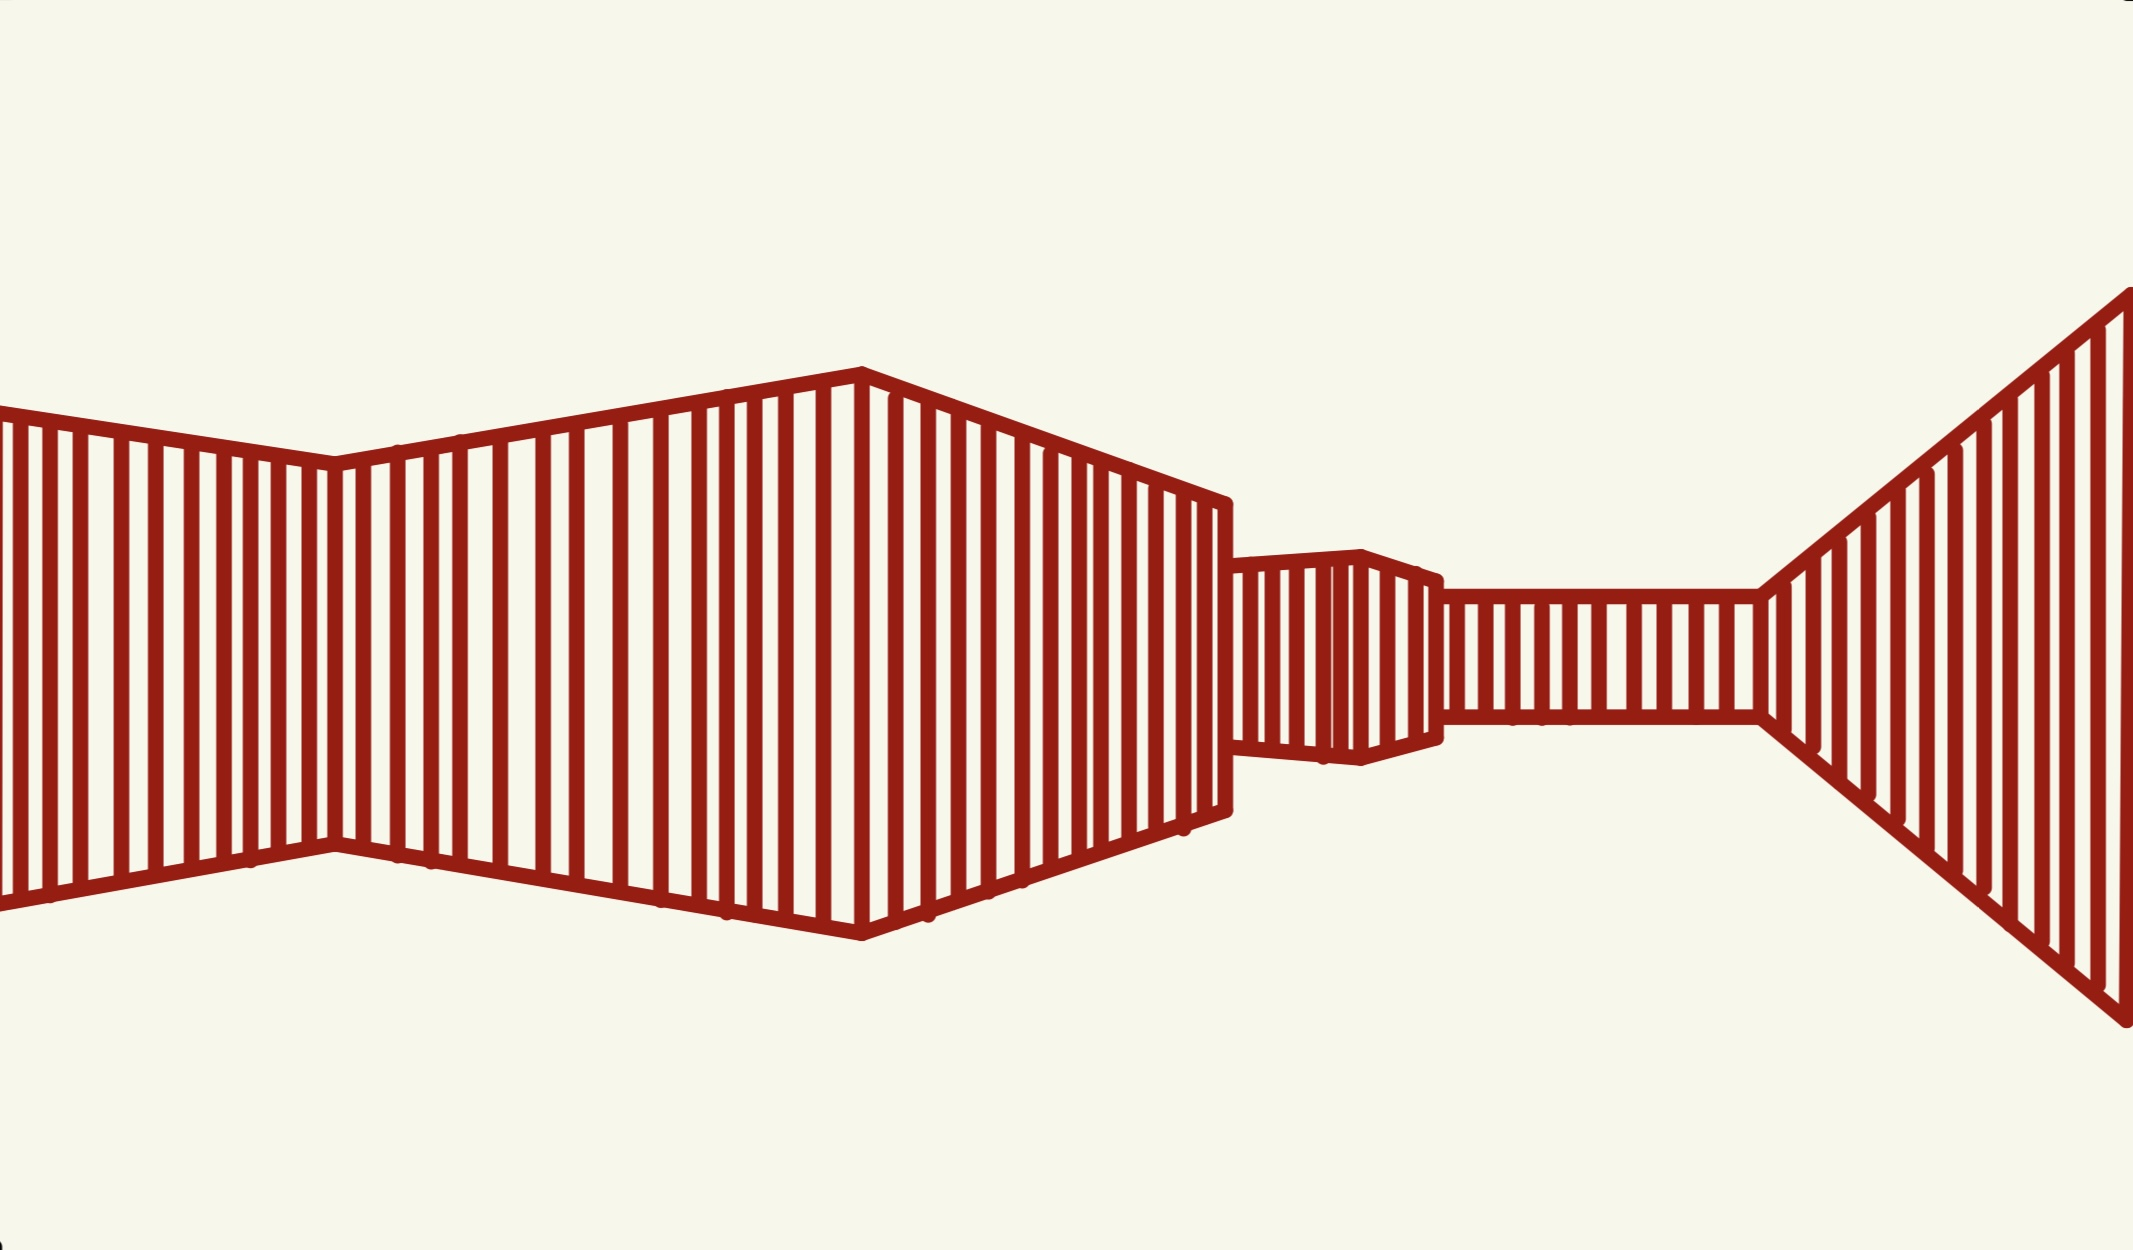
\includegraphics[width=0.6\textwidth]{images/rendu-historique.jpg}
    \end{figure}
\end{frame}

\begin{frame}
    \frametitle{Différentes stratégie pour un rendu 3D \\
                \small DDA}           
    \begin{block}{}
        \begin{itemize}
            \item Conçu pour la rasterisation de lignes
            \item Repose sur l'itération linéaire
            \item Employé pour déterminer où les rayons projetés intersectent avec les objets de l'environnement
        \end{itemize}
    \end{block}    
    \begin{figure}
        \centering
        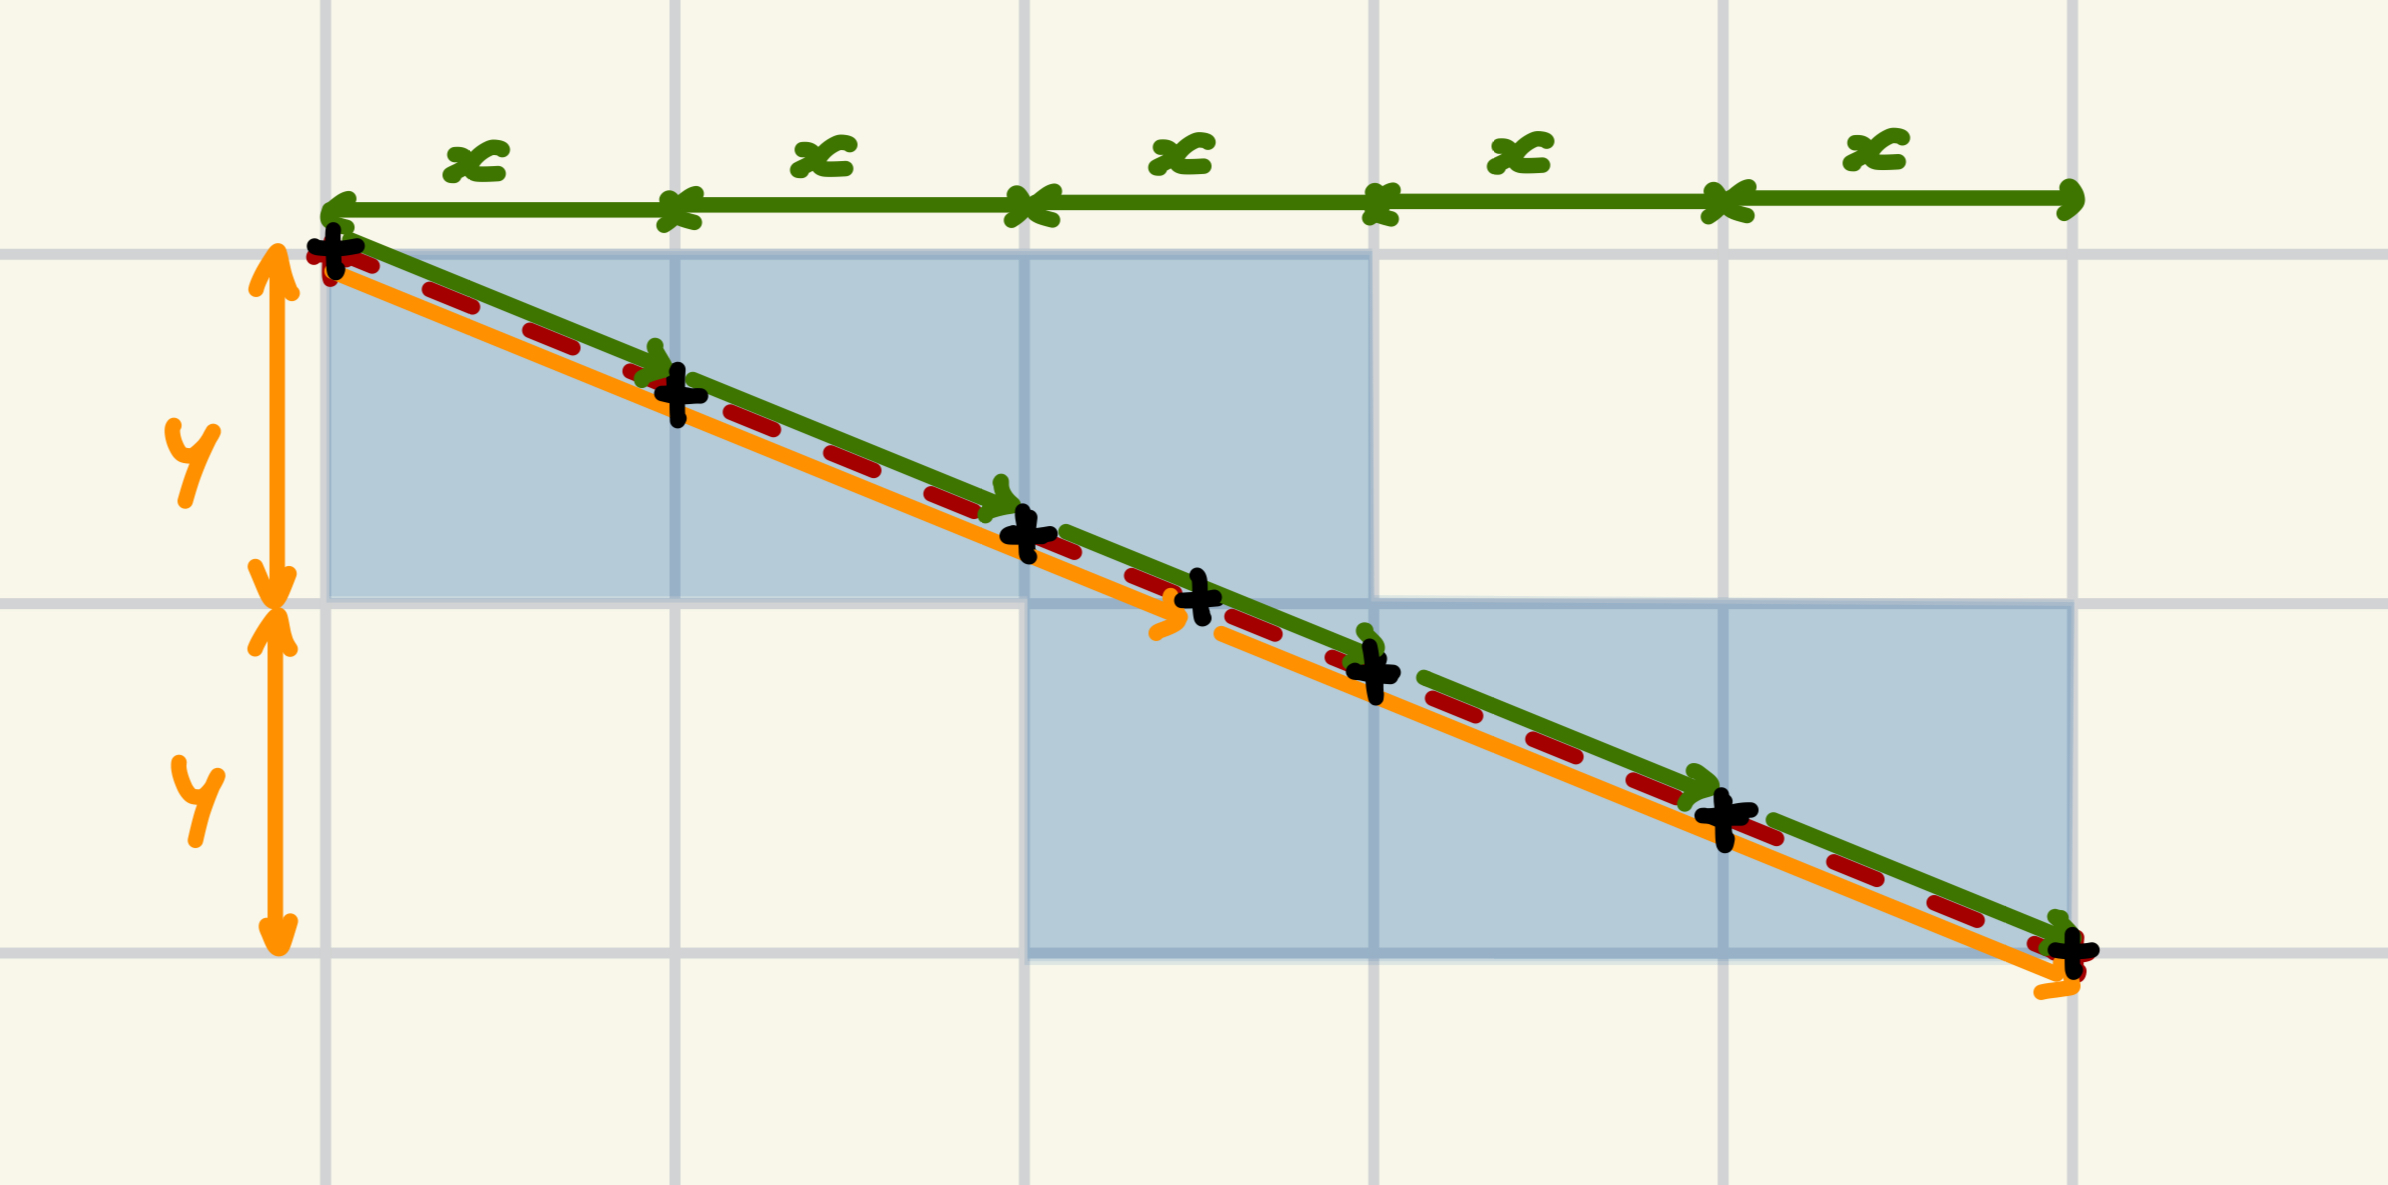
\includegraphics[width=0.7\textwidth]{images/DDA 0.jpg}
    \end{figure}
\end{frame}

\begin{frame}
    \frametitle{Différentes stratégie pour un rendu 3D \\
                \small DDA}           
    \begin{block}{Fonctionnement de DDA.}
        \begin{itemize}
            \item Déplacement vertical et horizontal d'une unité.
            \item Comparaison entre les distances parcourus sur le segment.
            \item Choix de la distance la plus petite.
        \end{itemize}
    \end{block}    
    \begin{figure}
        \centering
        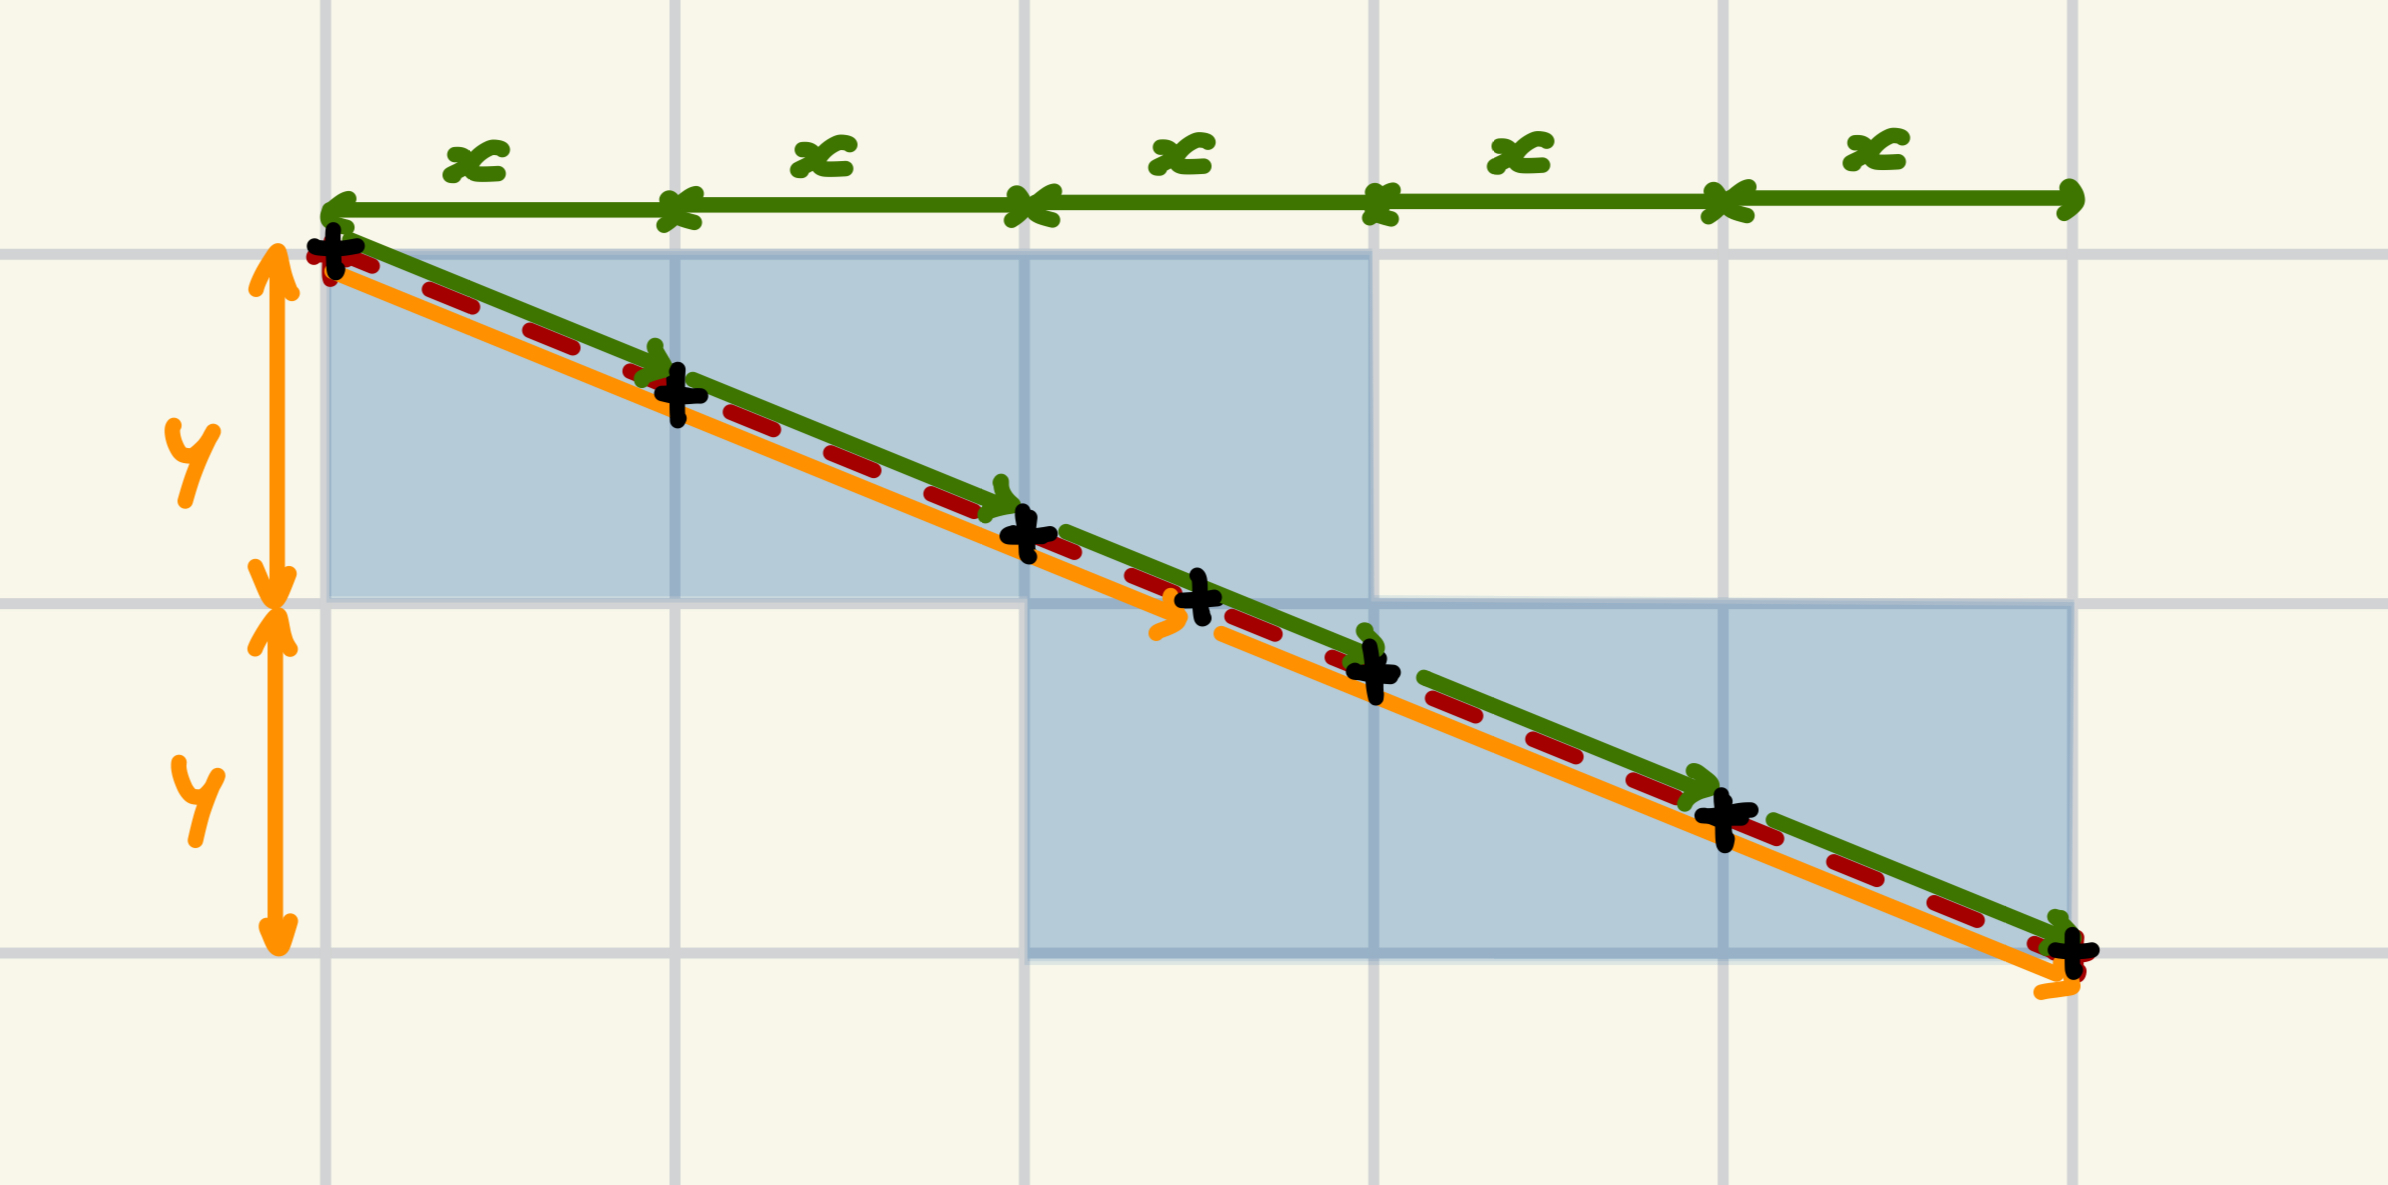
\includegraphics[width=0.7\textwidth]{images/DDA 0.jpg}
    \end{figure}
\end{frame}

\begin{frame}
    \frametitle{Différentes stratégie pour un rendu 3D \\
                \small DDA}           
    \begin{block}{Fonctionnement de DDA.}
        \begin{itemize}
            \item Déplacement vertical et horizontal d'une unité.
            \item Comparaison entre les distances parcourus sur le segment.
            \item Choix de la distance la plus petite.
        \end{itemize}
    \end{block}    
    \begin{figure}
        \centering
        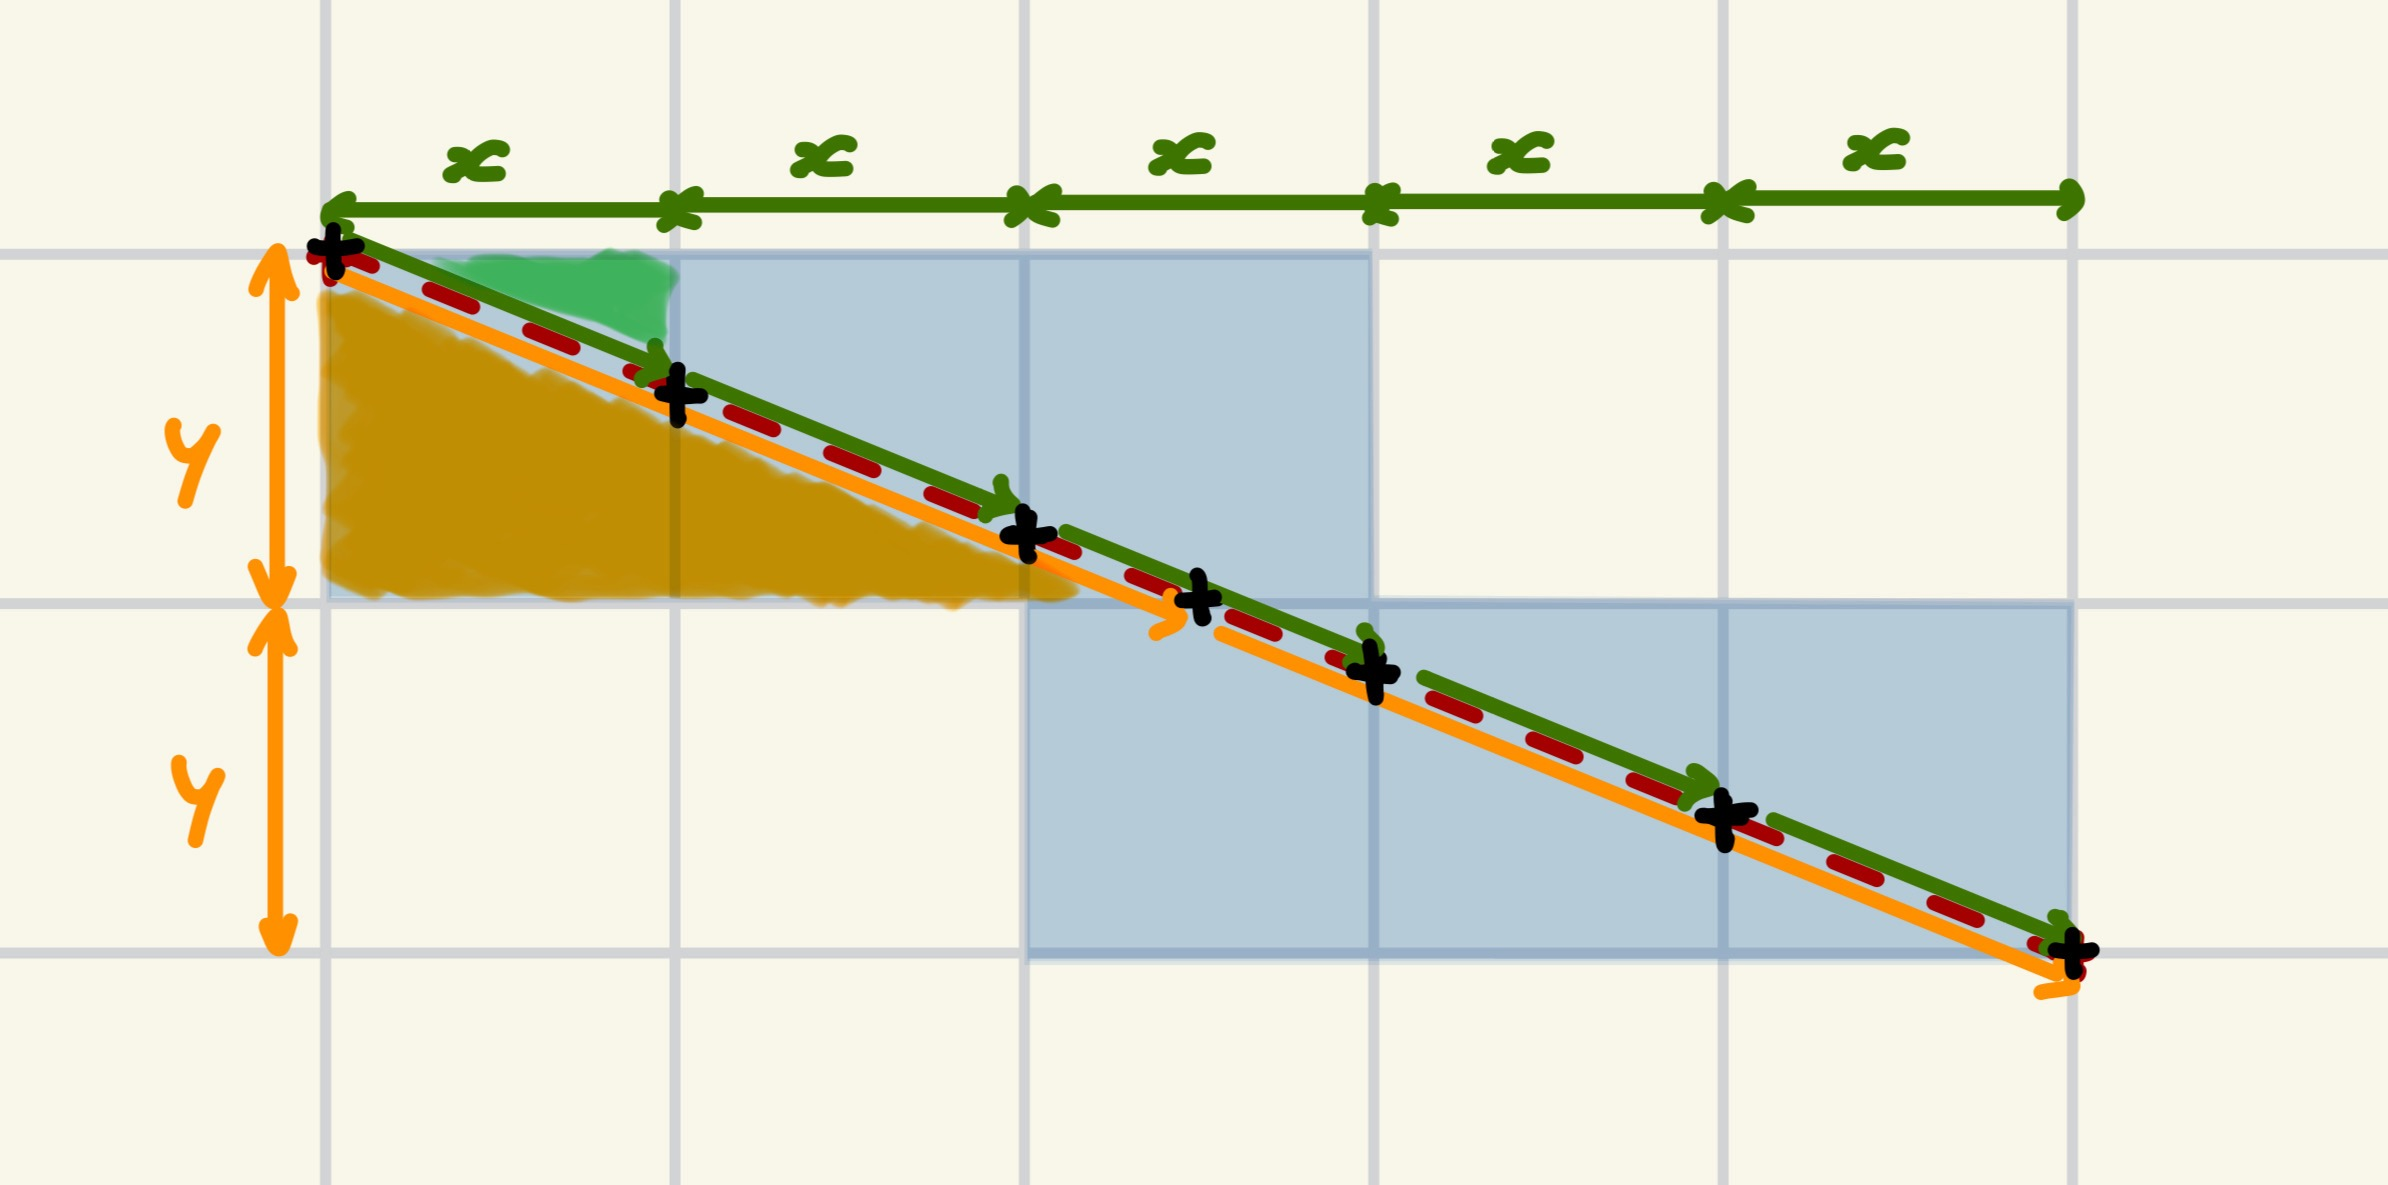
\includegraphics[width=0.7\textwidth]{images/DDA 1.jpg}
    \end{figure}
\end{frame}

\begin{frame}
    \frametitle{Différentes stratégie pour un rendu 3D \\
                \small DDA}           
    \begin{block}{Fonctionnement de DDA.}
        \begin{itemize}
            \item Déplacement vertical et horizontal d'une unité.
            \item Comparaison entre les distances parcourus sur le segment.
            \item Choix de la distance la plus petite.
        \end{itemize}
    \end{block}    
    \begin{figure}
        \centering
        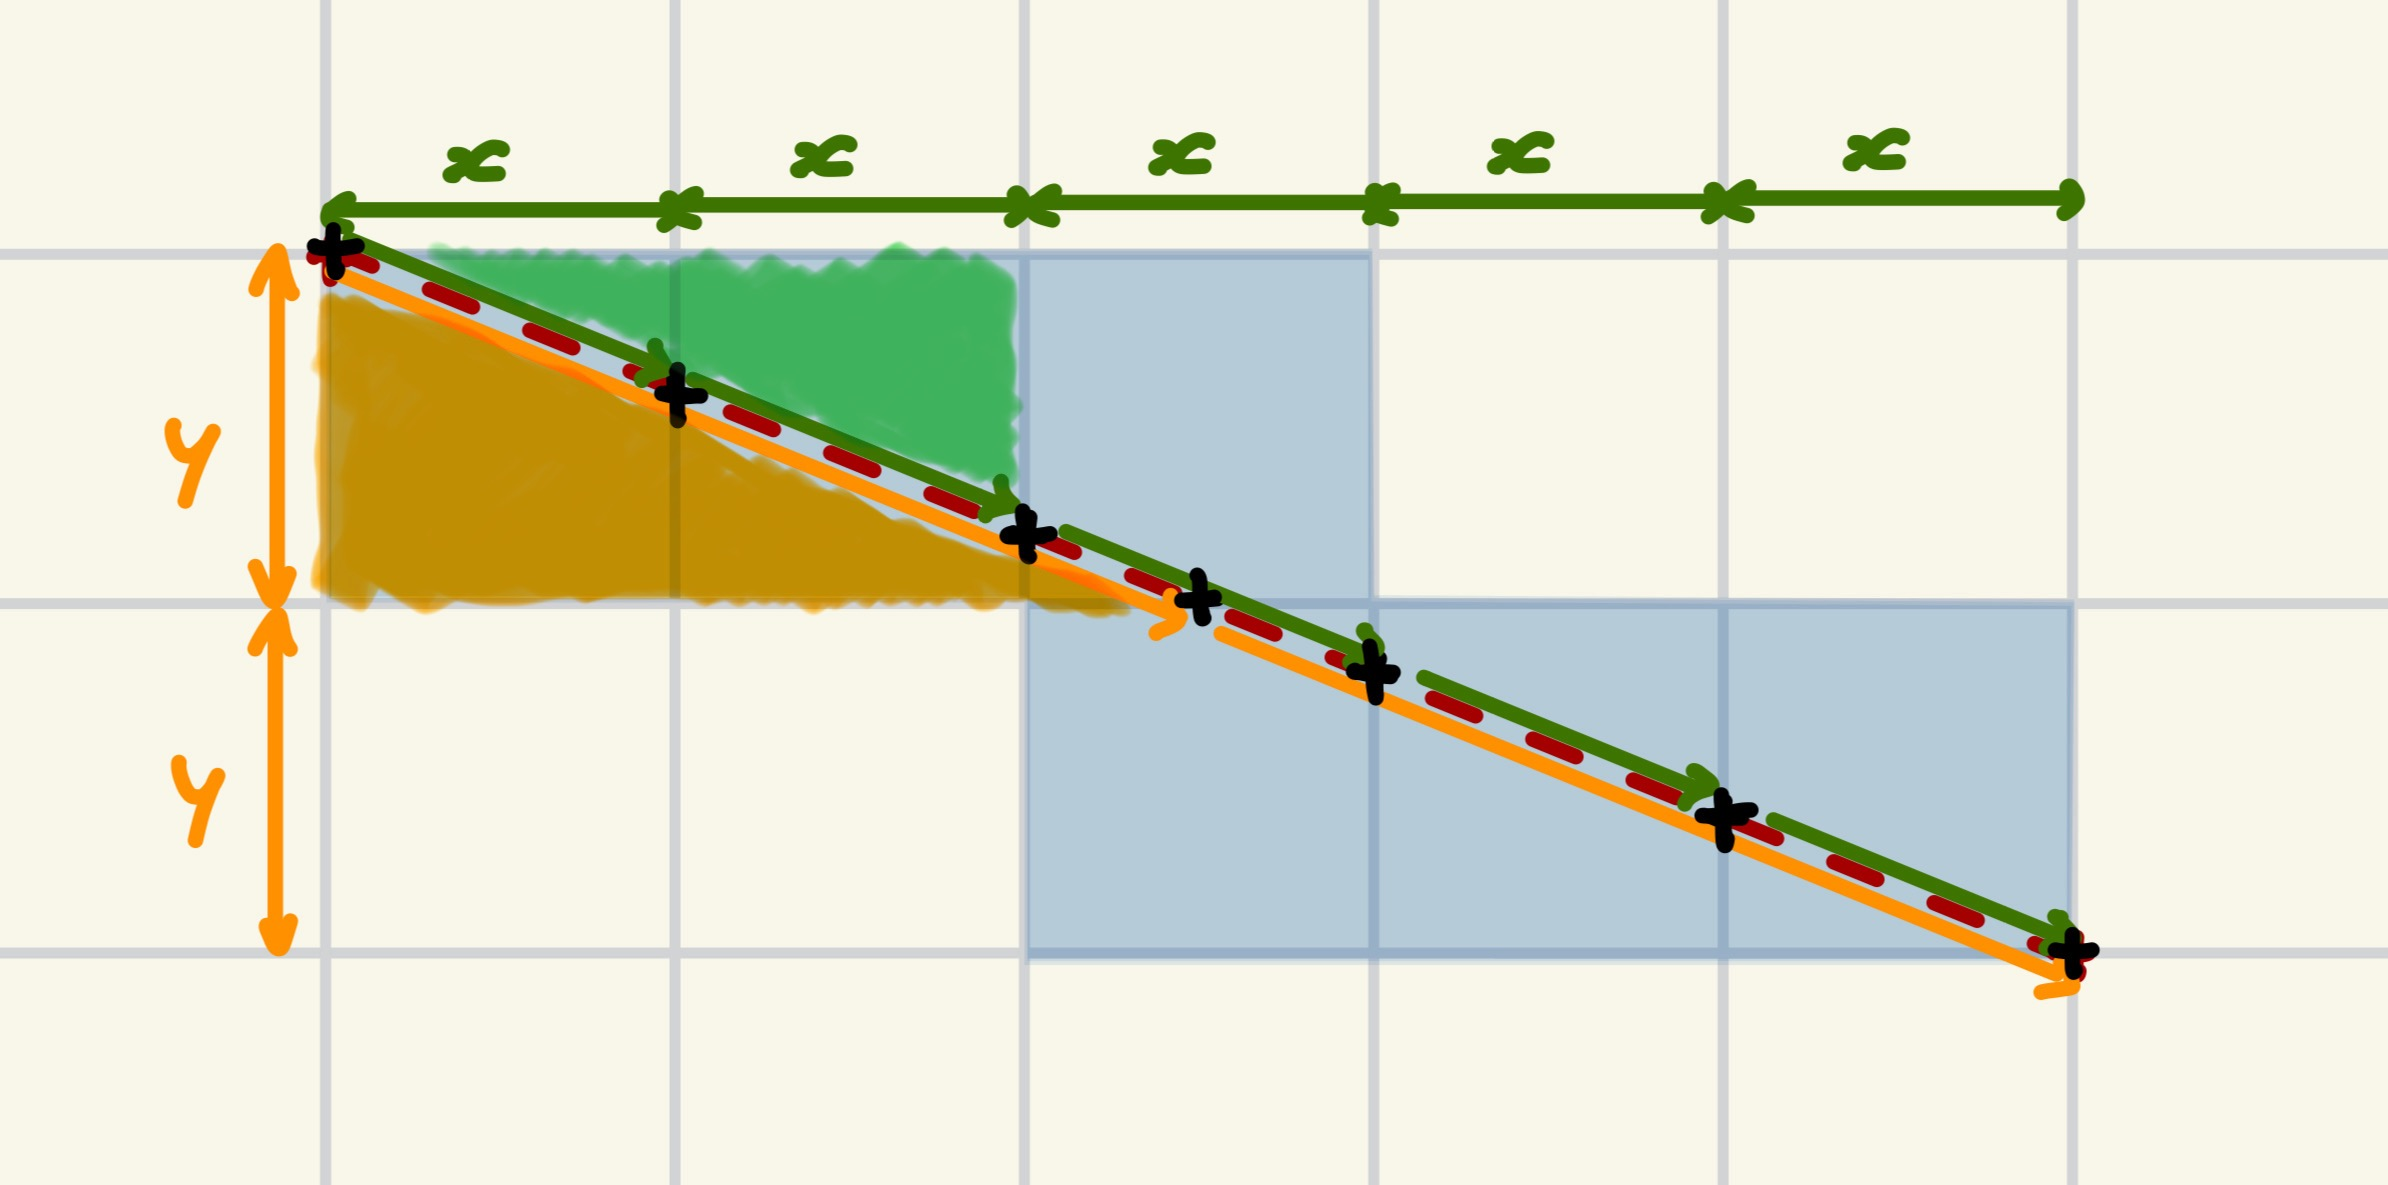
\includegraphics[width=0.7\textwidth]{images/DDA 2.jpg}
    \end{figure}
\end{frame}

\begin{frame}
    \frametitle{Différentes stratégie pour un rendu 3D \\
                \small DDA}           
    \begin{block}{Fonctionnement de DDA.}
        \begin{itemize}
            \item Déplacement vertical et horizontal d'une unité.
            \item Comparaison entre les distances parcourus sur le segment.
            \item Choix de la distance la plus petite.
        \end{itemize}
    \end{block}    
    \begin{figure}
        \centering
        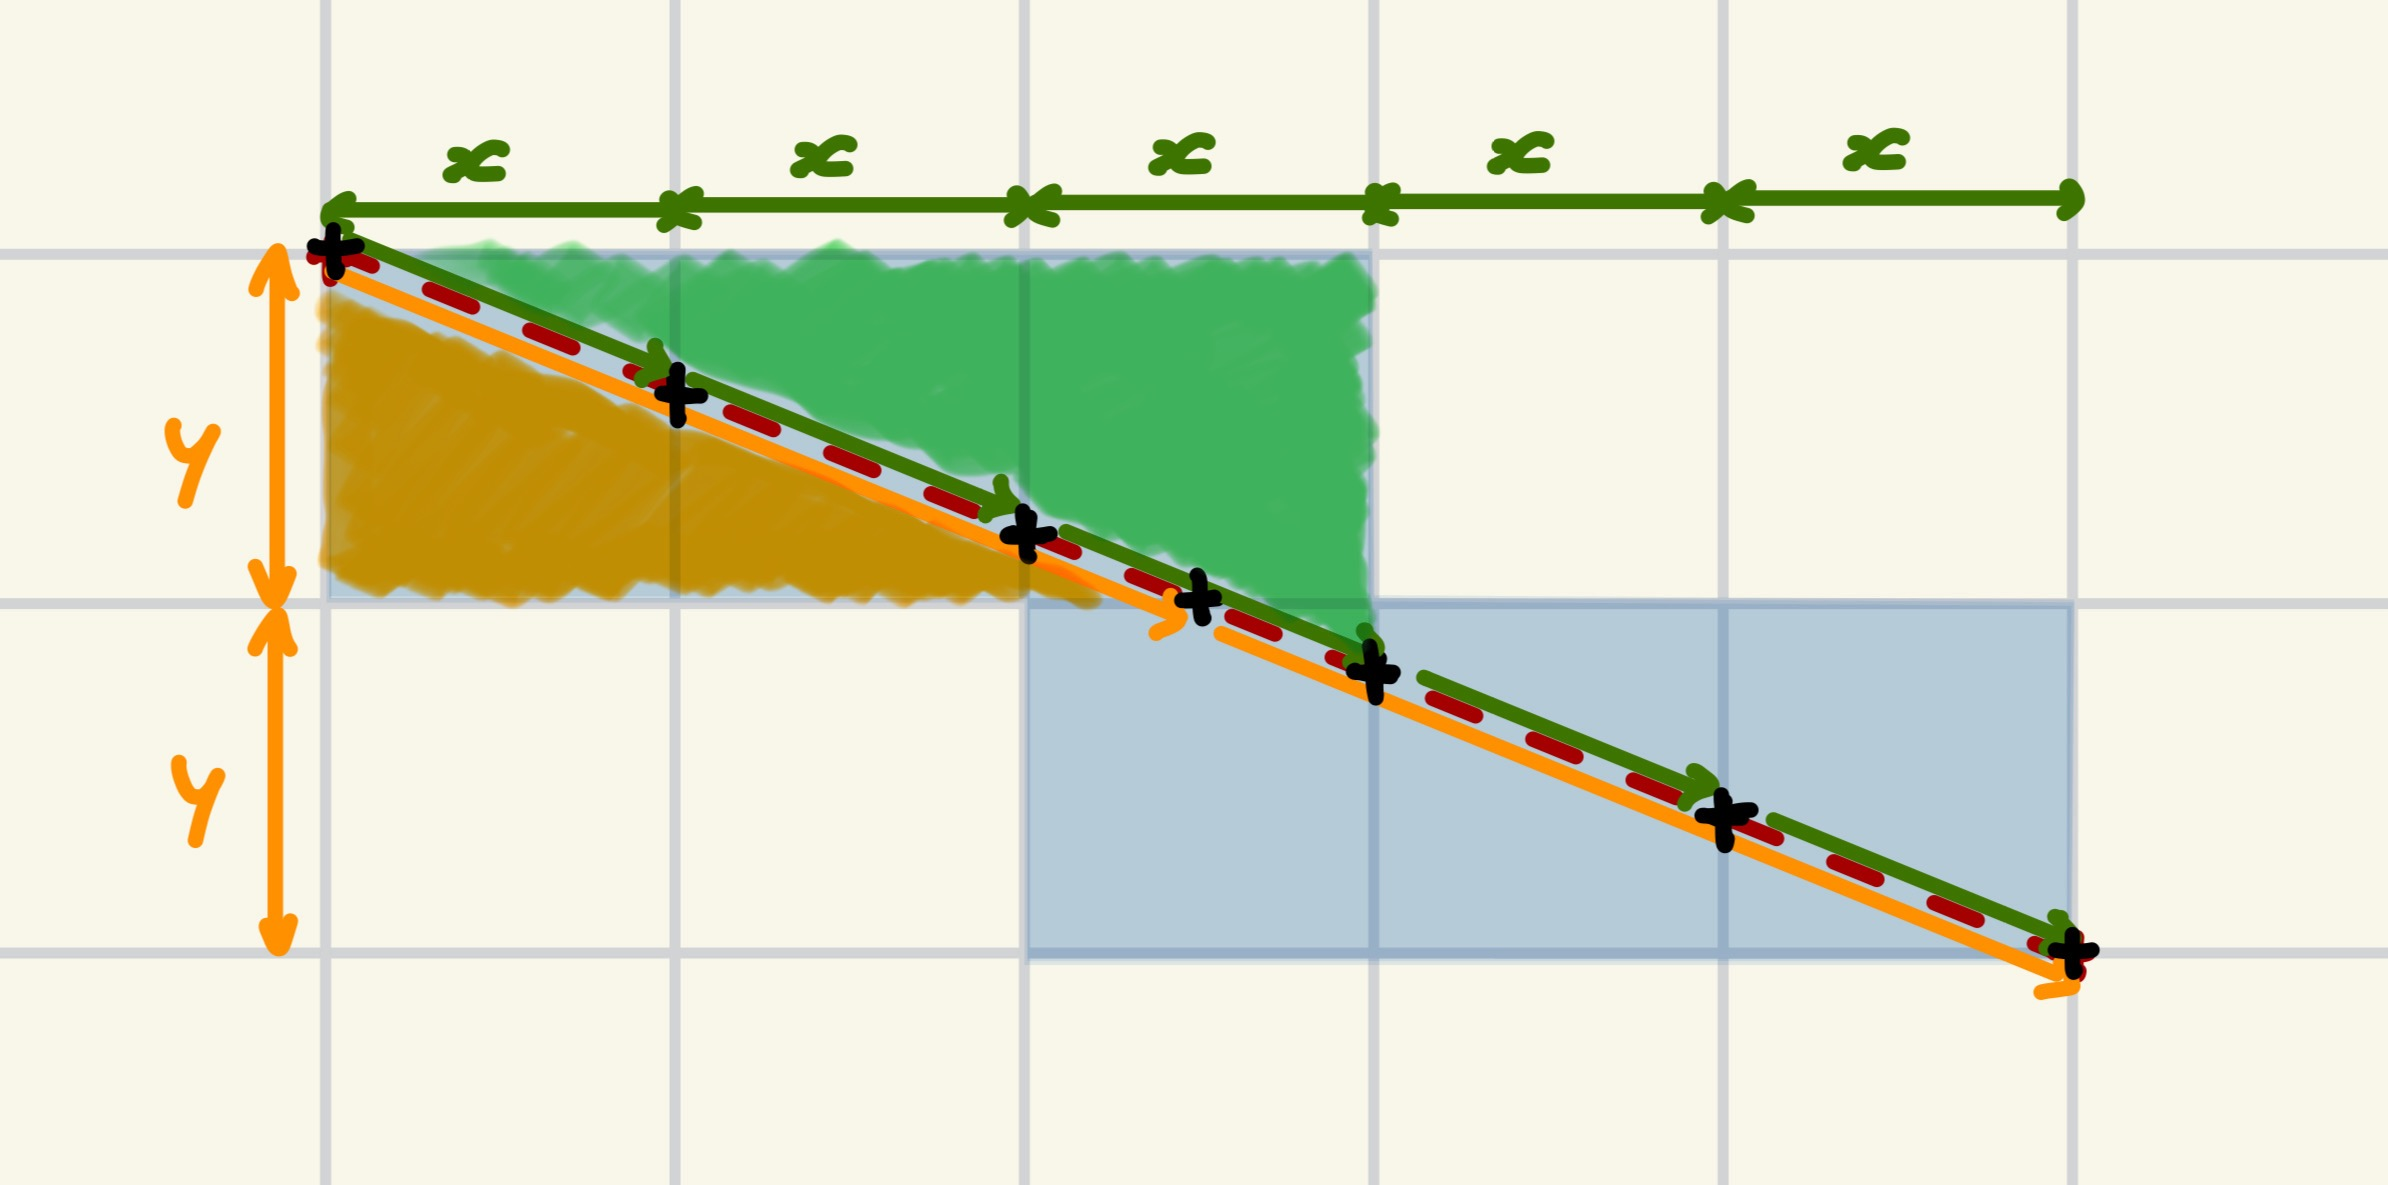
\includegraphics[width=0.7\textwidth]{images/DDA 3.jpg}
    \end{figure}
\end{frame}

\begin{frame}
    \frametitle{Différentes stratégie pour un rendu 3D \\
                \small DDA}           
    \begin{block}{Fonctionnement de DDA.}
        \begin{itemize}
            \item Déplacement vertical et horizontal d'une unité.
            \item Comparaison entre les distances parcourus sur le segment.
            \item Choix de la distance la plus petite.
        \end{itemize}
    \end{block}    
    \begin{figure}
        \centering
        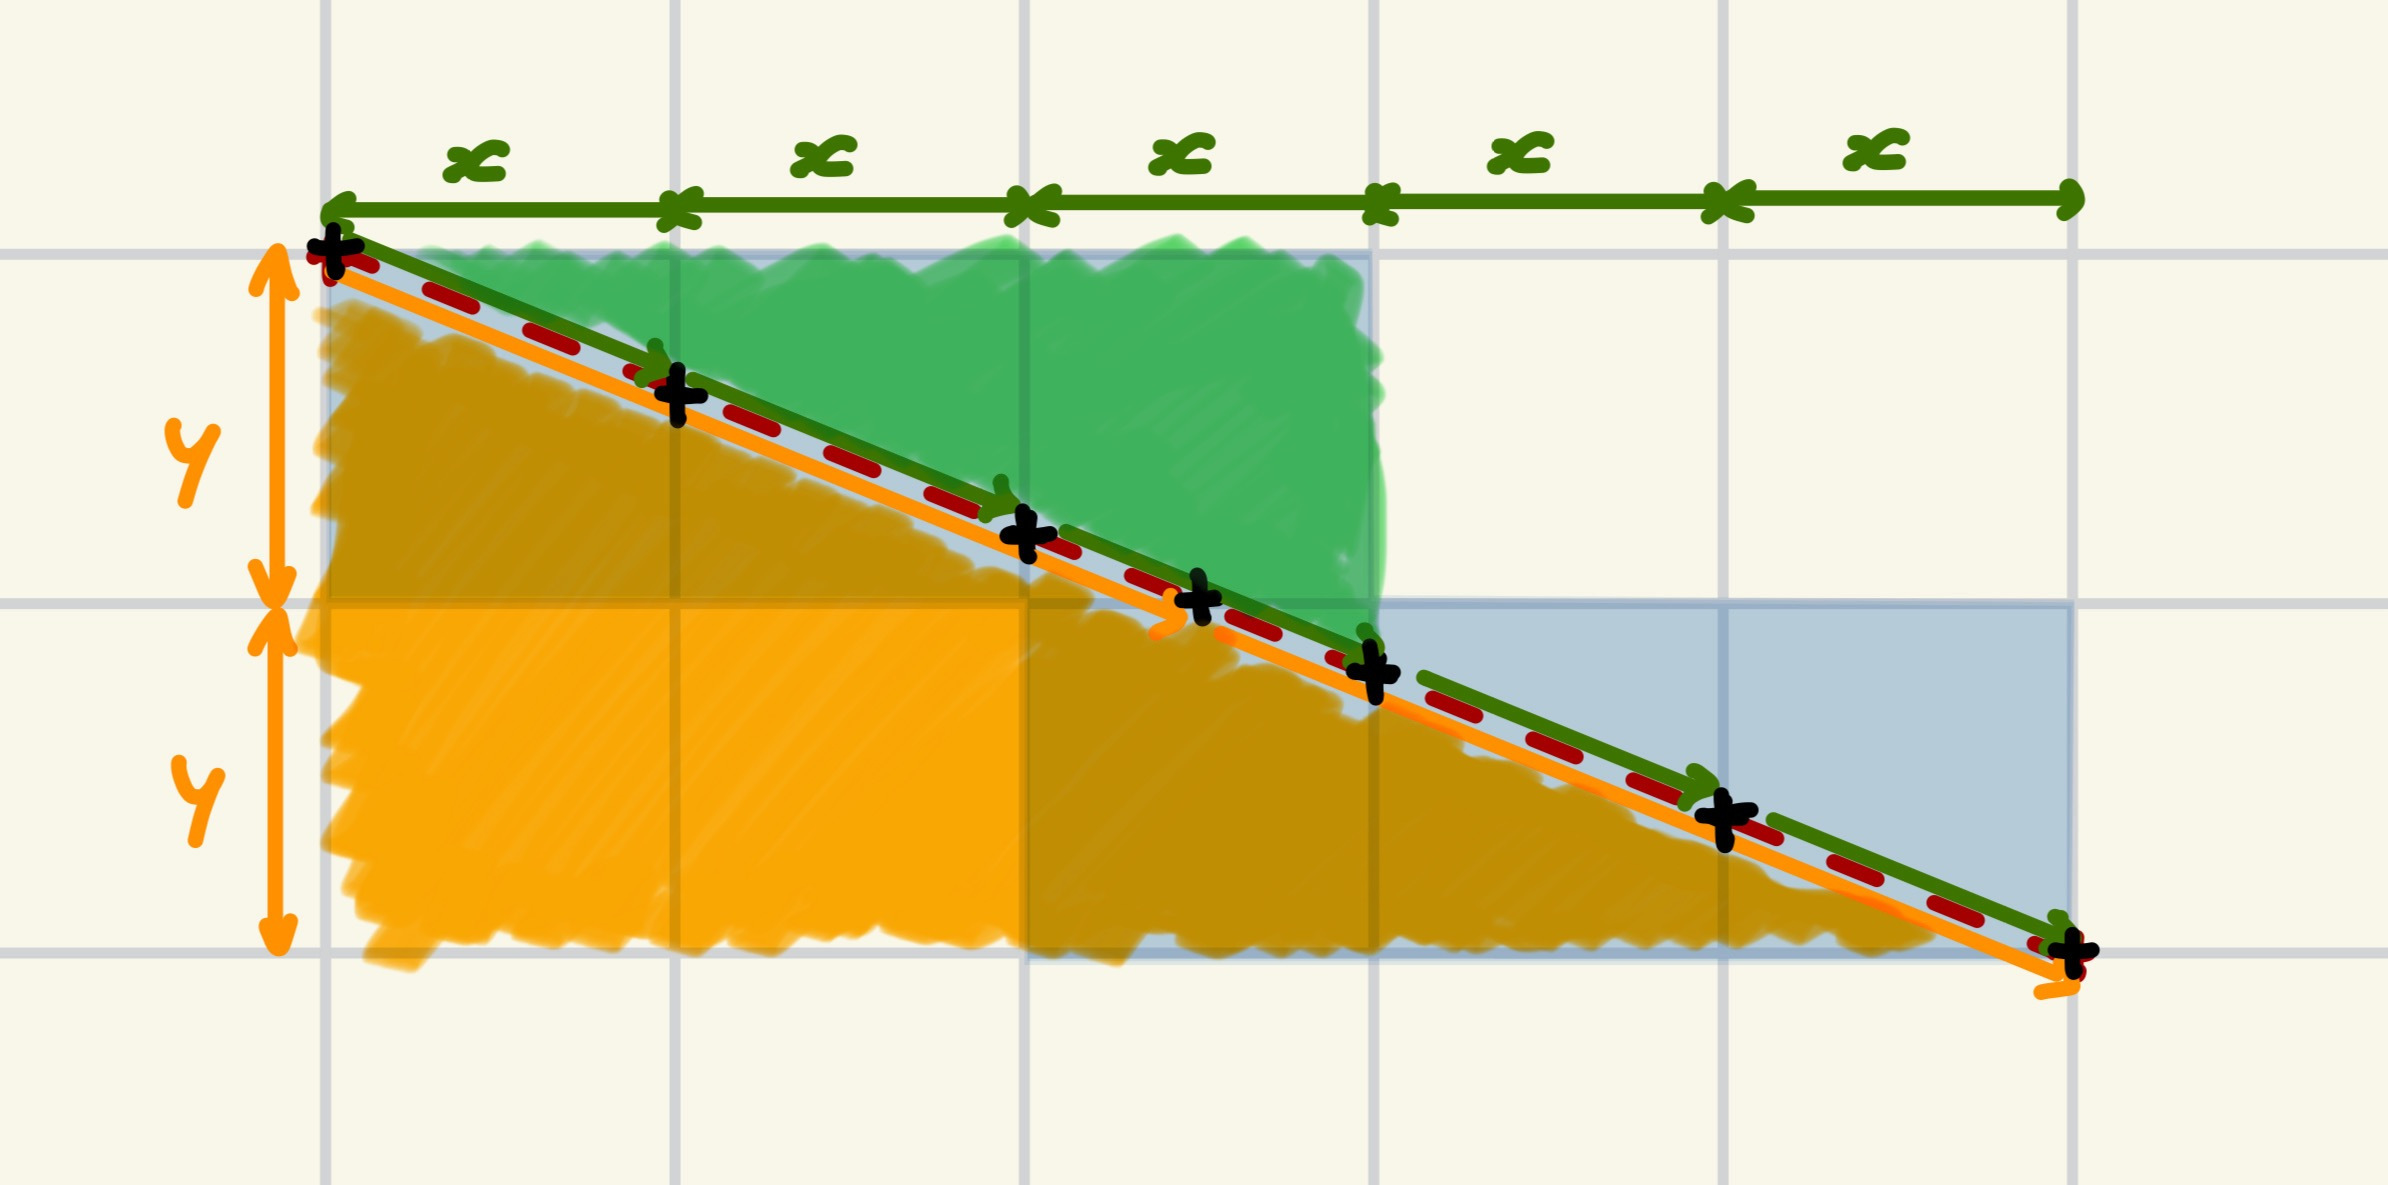
\includegraphics[width=0.7\textwidth]{images/DDA 4.jpg}
    \end{figure}
\end{frame}

\begin{frame}
    \frametitle{Différentes stratégie pour un rendu 3D \\
                \small DDA}           
    \begin{block}{Fonctionnement de DDA.}
        \begin{itemize}
            \item Déplacement vertical et horizontal d'une unité.
            \item Comparaison entre les distances parcourus sur le segment.
            \item Choix de la distance la plus petite.
        \end{itemize}
    \end{block}    
    \begin{figure}
        \centering
        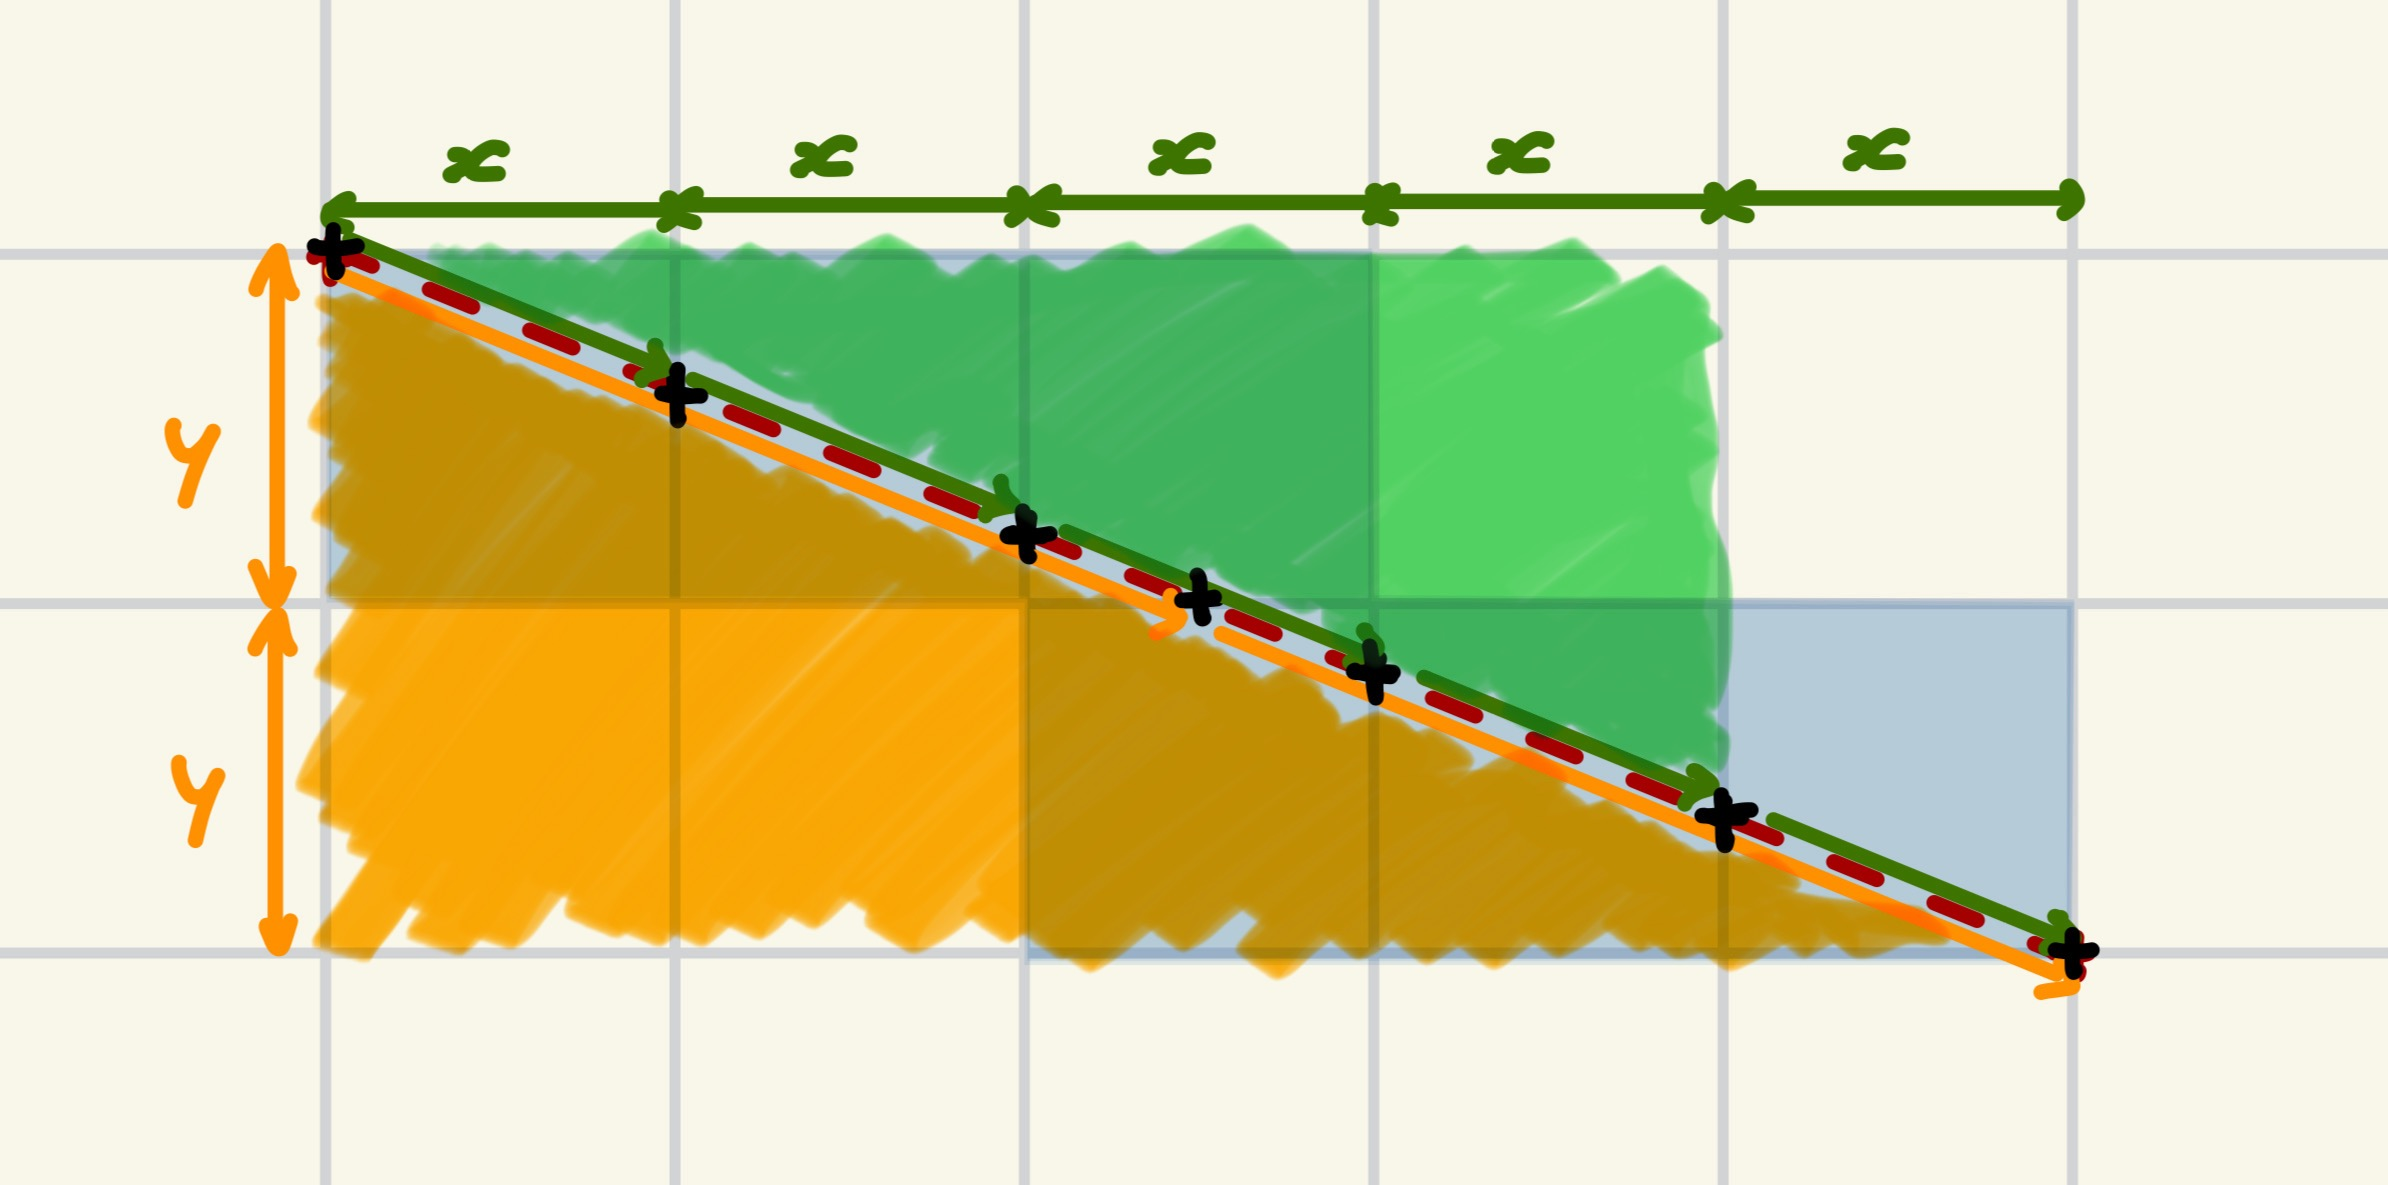
\includegraphics[width=0.7\textwidth]{images/DDA 5.jpg}
    \end{figure}
\end{frame}

\begin{frame}
    \frametitle{Différentes stratégie pour un rendu 3D \\
                \small DDA}           
    \begin{block}{Fonctionnement de DDA.}
        \begin{itemize}
            \item Déplacement vertical et horizontal d'une unité.
            \item Comparaison entre les distances parcourus sur le segment.
            \item Choix de la distance la plus petite.
        \end{itemize}
    \end{block}    
    \begin{figure}
        \centering
        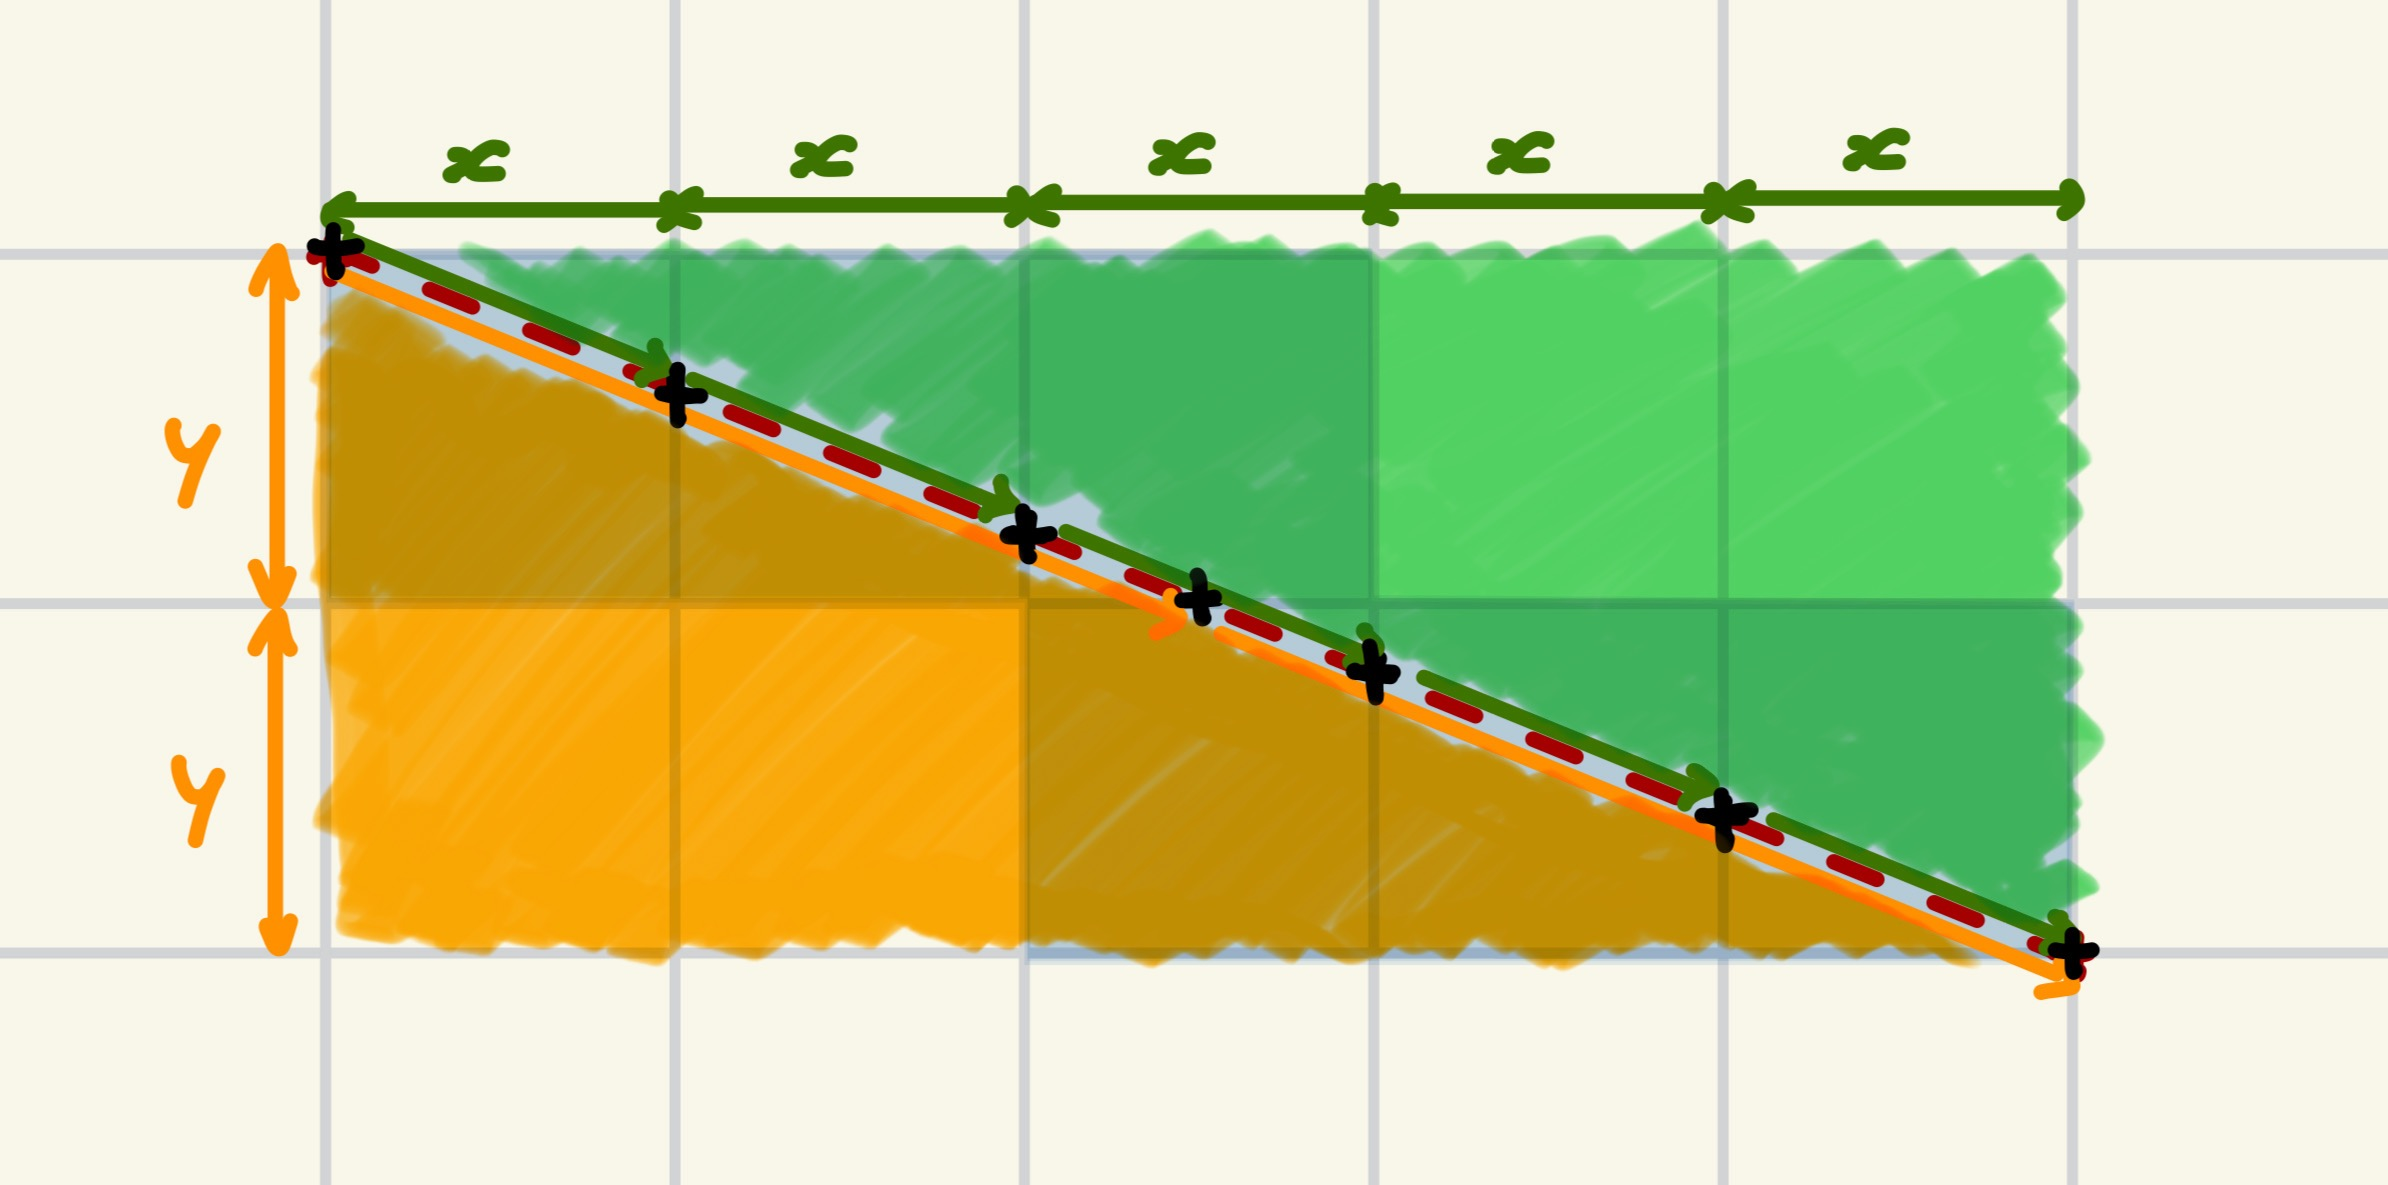
\includegraphics[width=0.7\textwidth]{images/DDA 6.jpg}
    \end{figure}
\end{frame}

% \begin{frame}
%     \frametitle{Différentes stratégie pour un rendu 3D \\
%                 \small DDA}           
%     \begin{block}{}
%         \begin{itemize}
%             \item Calcule l'emplacement correspondant sur l'autre axe en ajoutant un incrément constant
%             \item Utilisé pour trouver rapidement et précisément les intersections entre les rayons 
%             et les murs dans le raycasting
%         \end{itemize}
%         % L'algorithme DDA est historiquement conçu pour la rasterisation de 
%         % lignes, c'est-à-dire la conversion de lignes geometriques en ligne 
%         % visuelle composées de pixels alignés. Dans le contexte du raycasting, 
%         % DDA est employé pour déterminer où les rayons projetés à travers la 
%         % scène intersectent avec les objets de l'environnement, typiquement et 
%         % dans notre cas représenté par une grille de cellules. Le principe 
%         % fondamental de DDA repose sur l'itération linéaire. Plutôt que de 
%         % calculer chaque point le long d'une demie droite en utilisant des formules 
%         % de géométrie directe, ce qui pourrait être coûteux en termes de performances, 
%         % DDA avance par petits incr ́ements. Cela signifie que pour chaque
%         % pas sur l'axe le plus dominant (x ou y), DDA calcule l'emplacement 
%         % correspondant sur l'autre axe en ajoutant un incrément constant. 
%         % Cela se traduit par un parcours régulier et efficace le long de la 
%         % ligne en faisant des sauts à chaque intersection entre la demie 
%         % droite et la grille 2D. Dans le raycasting, DDA est utilisé pour 
%         % trouver rapidement et précisément les intersections entre les rayons 
%         % et les murs
%     \end{block}    
% \end{frame}

\begin{frame}
    \frametitle{Différentes stratégie pour un rendu 3D \\
                \small Approche moderne (Line Of Sight)}    
                
    
    \begin{block}{}
        \begin{itemize} 
            \item Envoyer un rayon pour chaque sommet de chaque mur
        \end{itemize}
%         Cette seconde approche s’approche des algorithme Line Of Sight et consiste
% a calculer la distance entre le joueur et chaque sommet de chaque mur.
% Pour ce faire on a pu recuperer l’algorithme DDA precedemment utilise
% pour le rendu des murs mais cette fois-ci en visant chaque sommets au lieu
% de viser chaque colonne de pixel. Cela permet theoriquement de reduire
% considerablement le nombre de calculs a effectuer.

    \end{block}    


    \begin{figure}
        \centering
        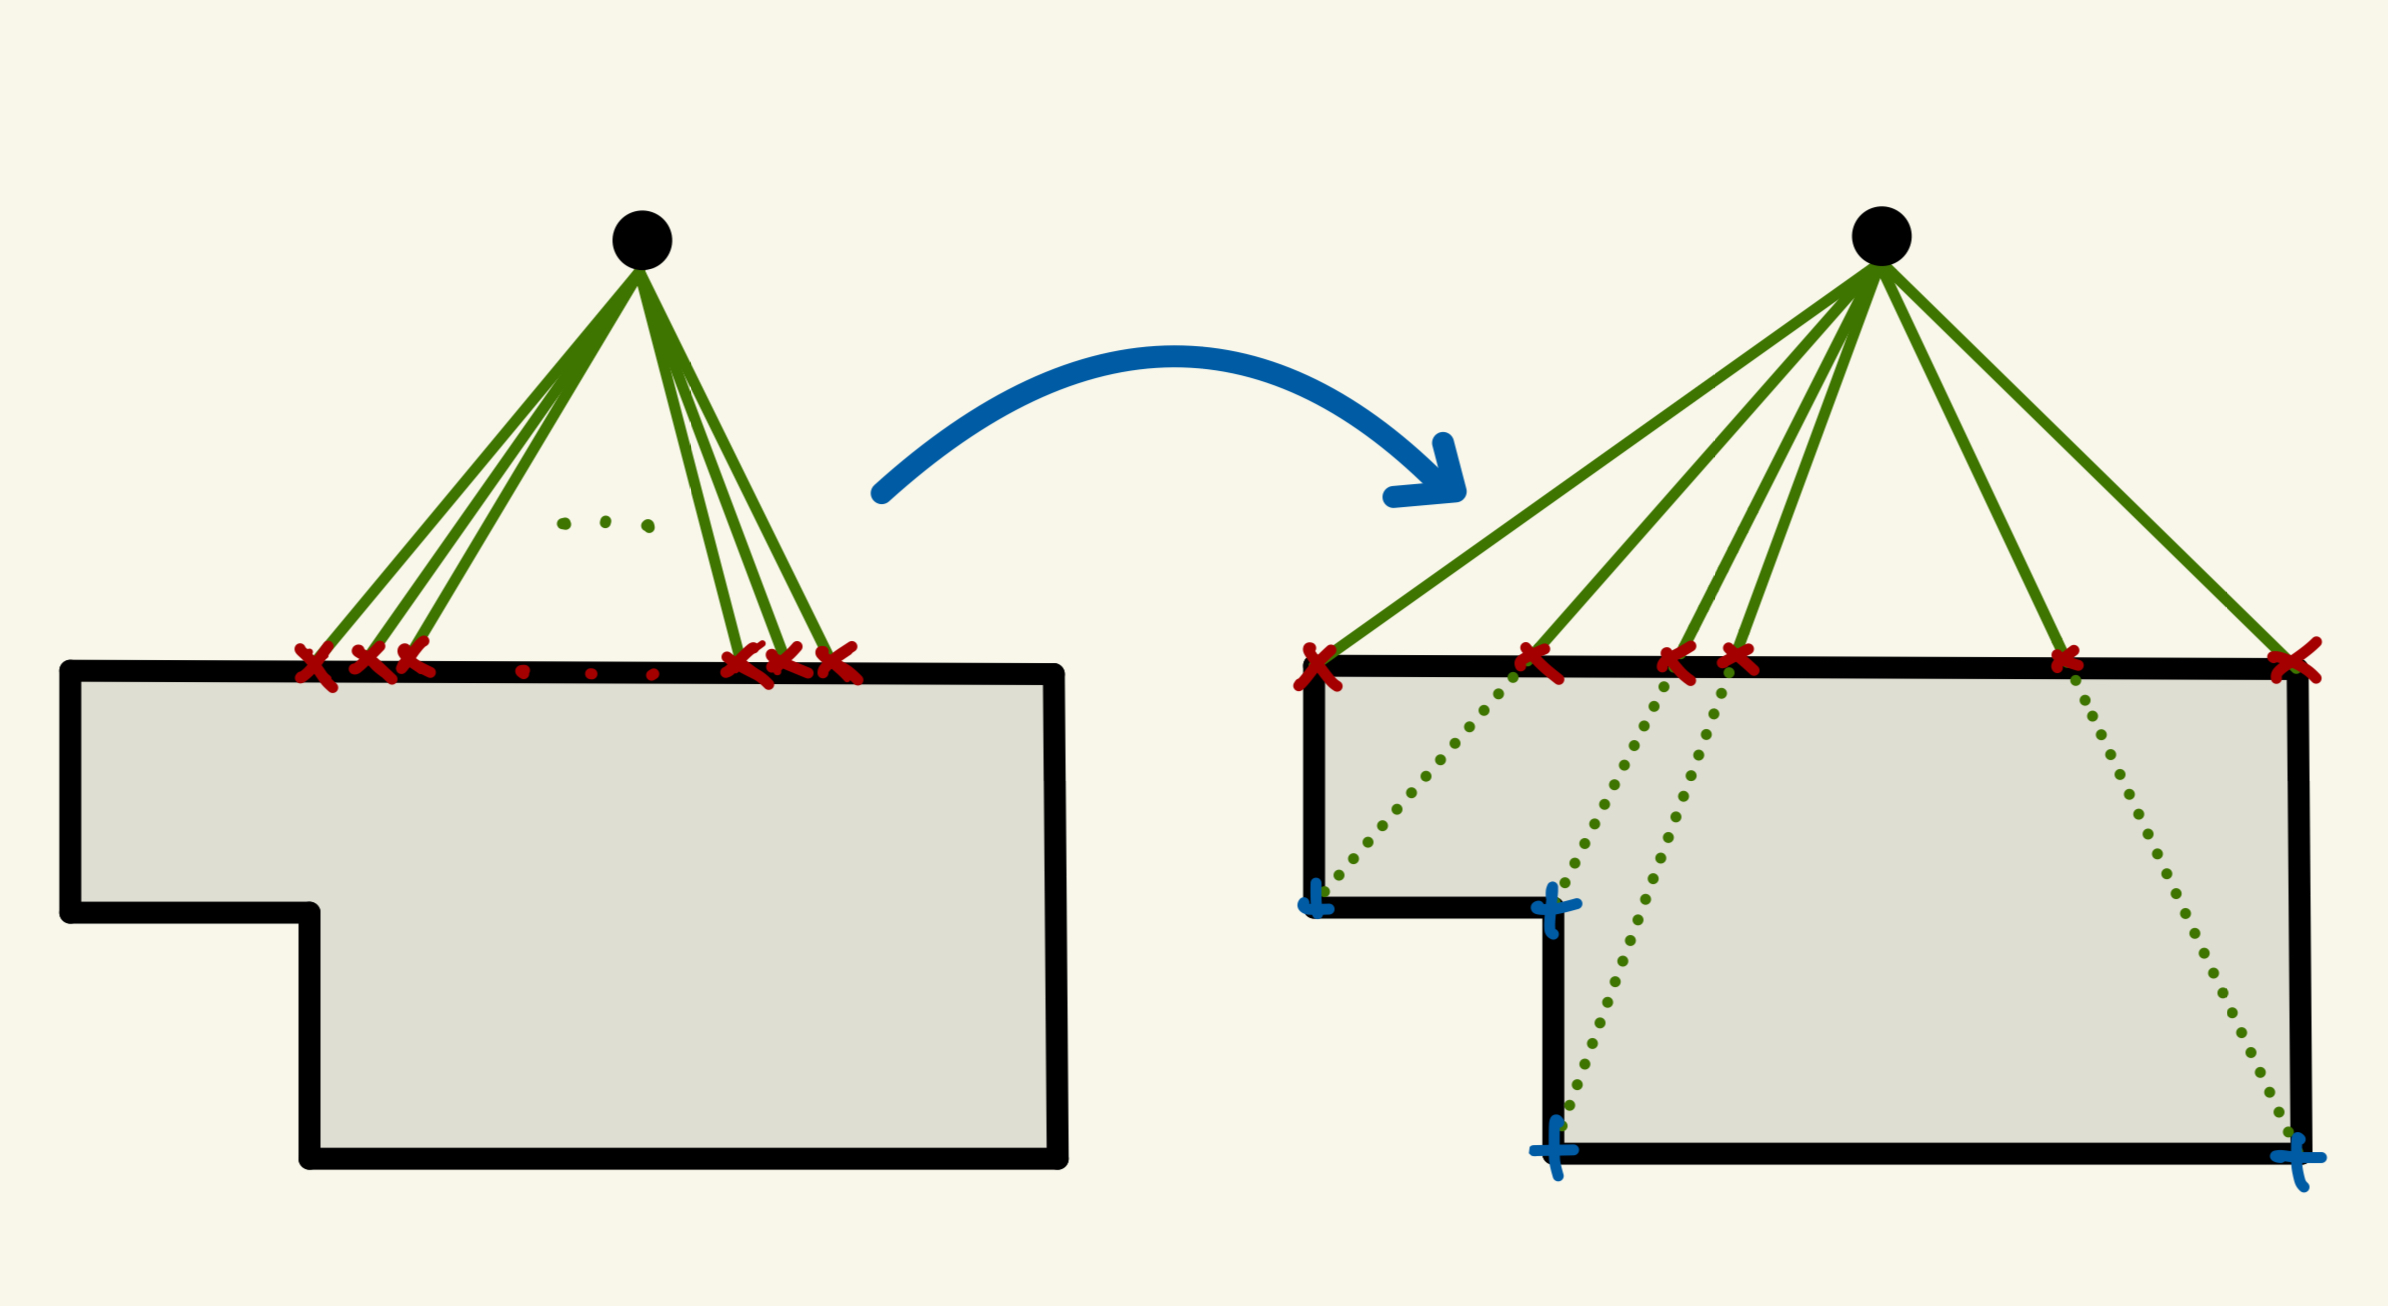
\includegraphics[width=0.8\textwidth]{images/comparaison-deux-methodes.jpeg}
    \end{figure}
\end{frame}


\section{Implémentation}

\subsection{Les rendus}

\begin{frame}
    \frametitle{Les rendus}
    \begin{block}{Deux étapes}
        \begin{itemize}
            \item Récupération des sommets triés 
            \item Envoie des rayons dans l'ordre avec DDA
        \end{itemize}
    \end{block}
    \begin{figure}
        \centering
        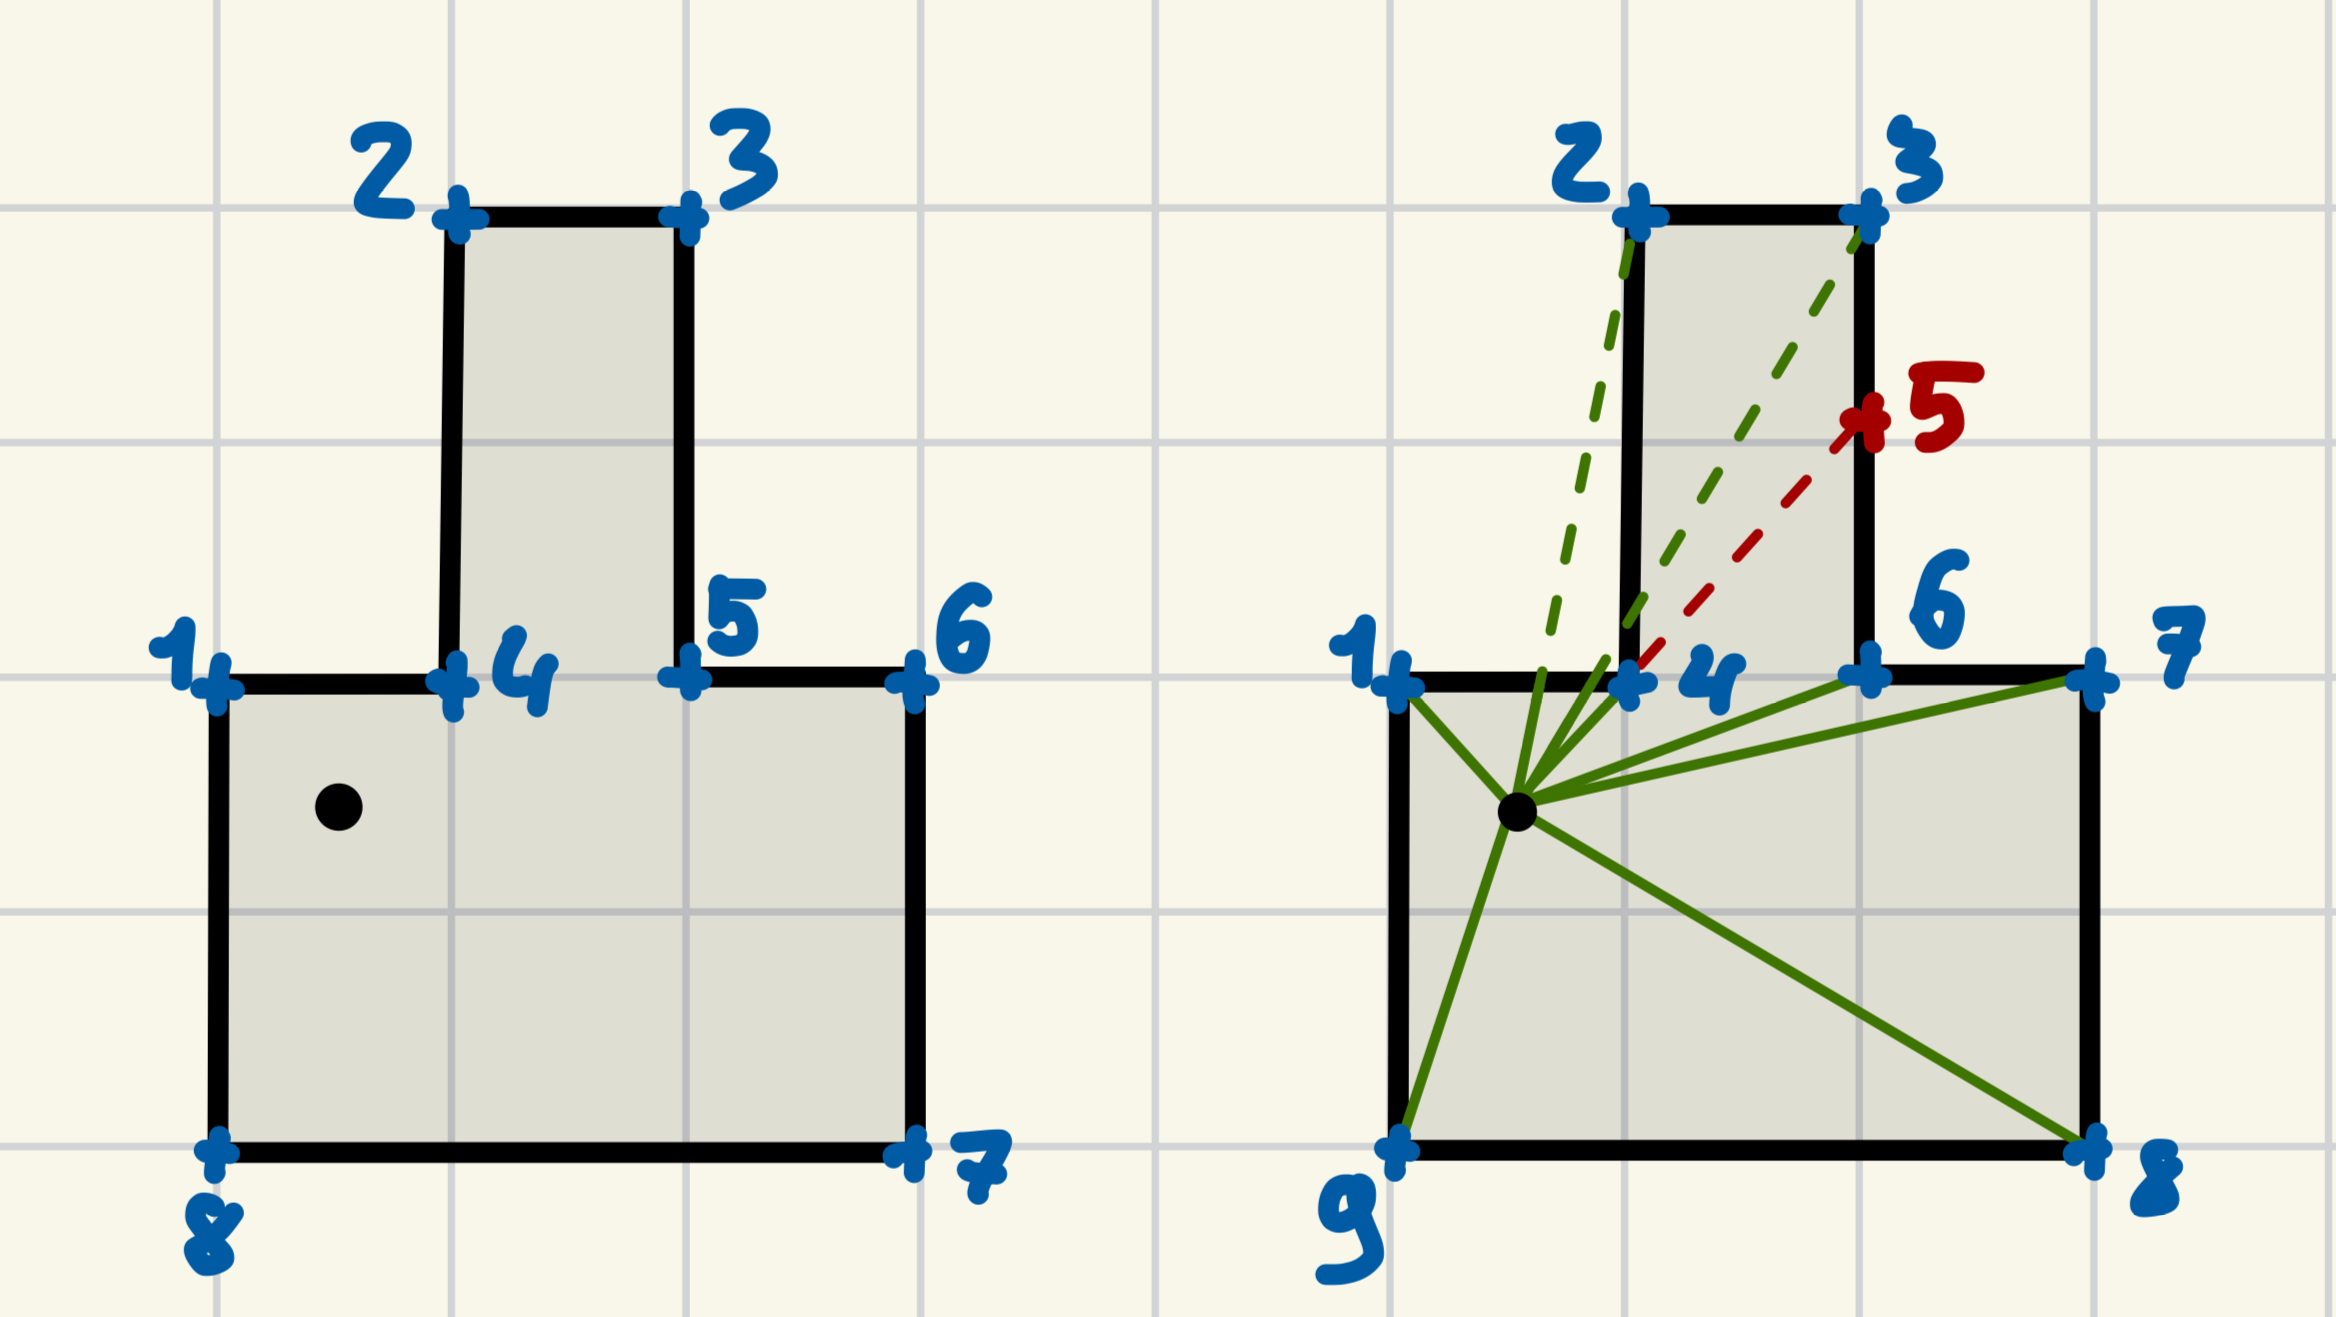
\includegraphics[width=0.7\textwidth]{images/envoie-rayon-ordre.jpg}
    \end{figure}
\end{frame}

\begin{frame}
    \frametitle{Les rendus}
    \begin{block}{Trois cas possibles}
        \begin{itemize}
            \item Le sommet est atteint et on arrête le rayon. 
            \item Le sommet n'est pas atteint donc on arrête le rayon.
            \item Le sommet est atteint mais on continue le rayon.
        \end{itemize}
    \end{block}
    \begin{figure}
        \centering
        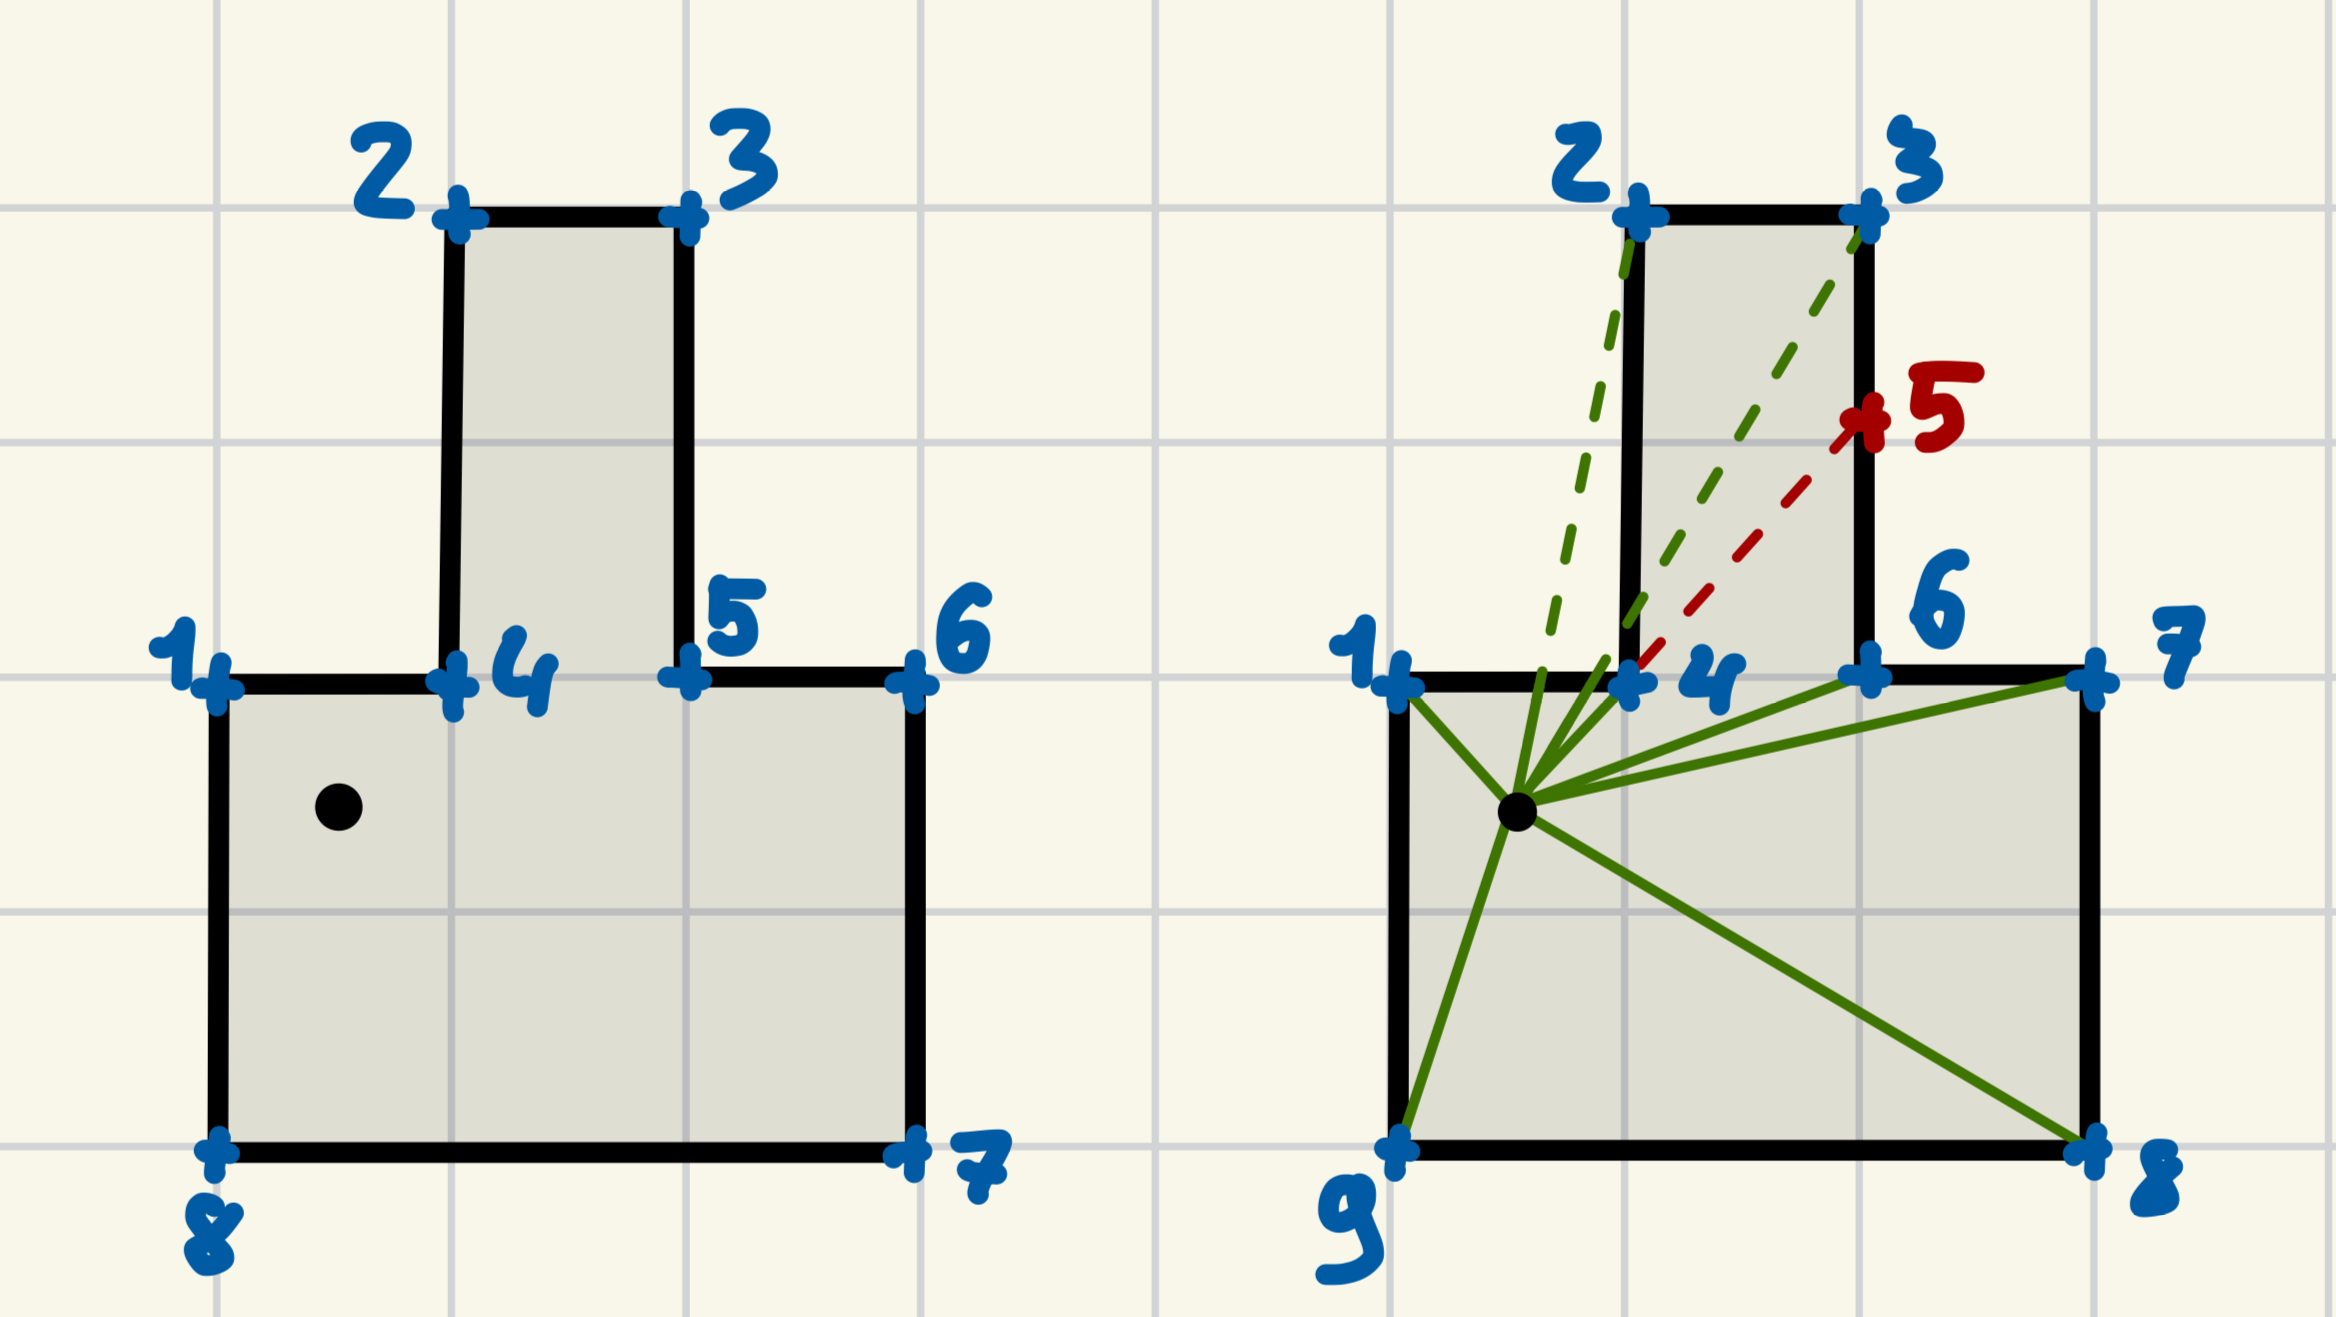
\includegraphics[width=0.7\textwidth]{images/envoie-rayon-ordre.jpg}
    \end{figure}
\end{frame}

% \begin{frame}
%     \frametitle{Les rendus}
%     \begin{block}{Projection des sommets}
%         \begin{itemize}
%             \item Déterminer la hauteur du segment (sommet en 3D) et sa position.
%         \end{itemize}
%     \end{block}
%     \begin{figure}
%         \centering
%         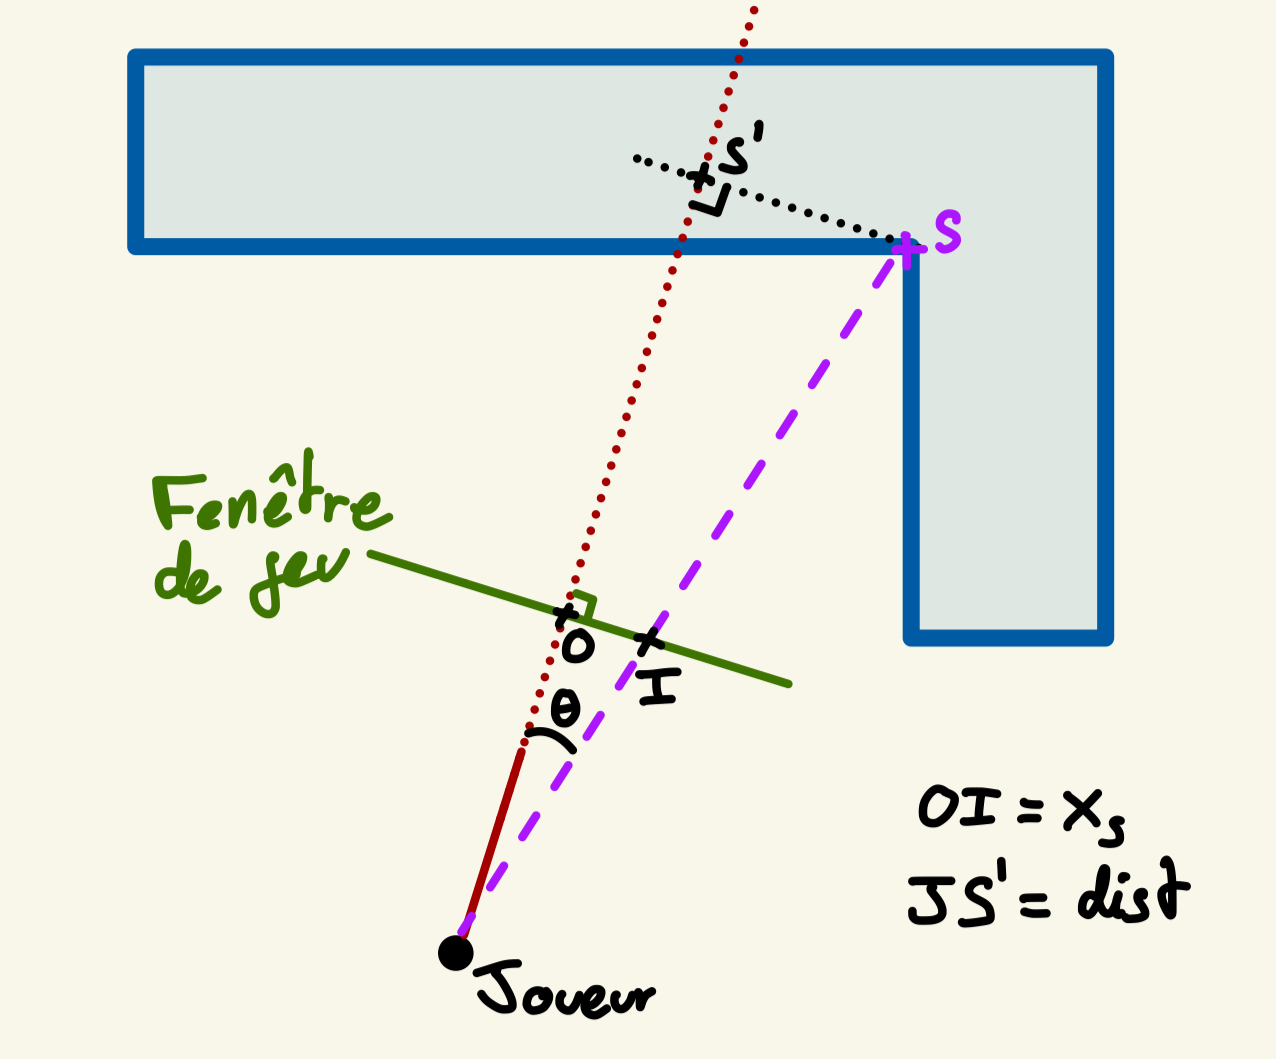
\includegraphics[width=0.7\textwidth]{images/shemaLanceRayon01.jpeg}
%     \end{figure}
% \end{frame}

\begin{frame}
    \frametitle{Les rendus}
    \begin{block}{}
        \begin{itemize}
            \item Résultat sans textures.
        \end{itemize}
    \end{block}
    \begin{figure}
        \centering
        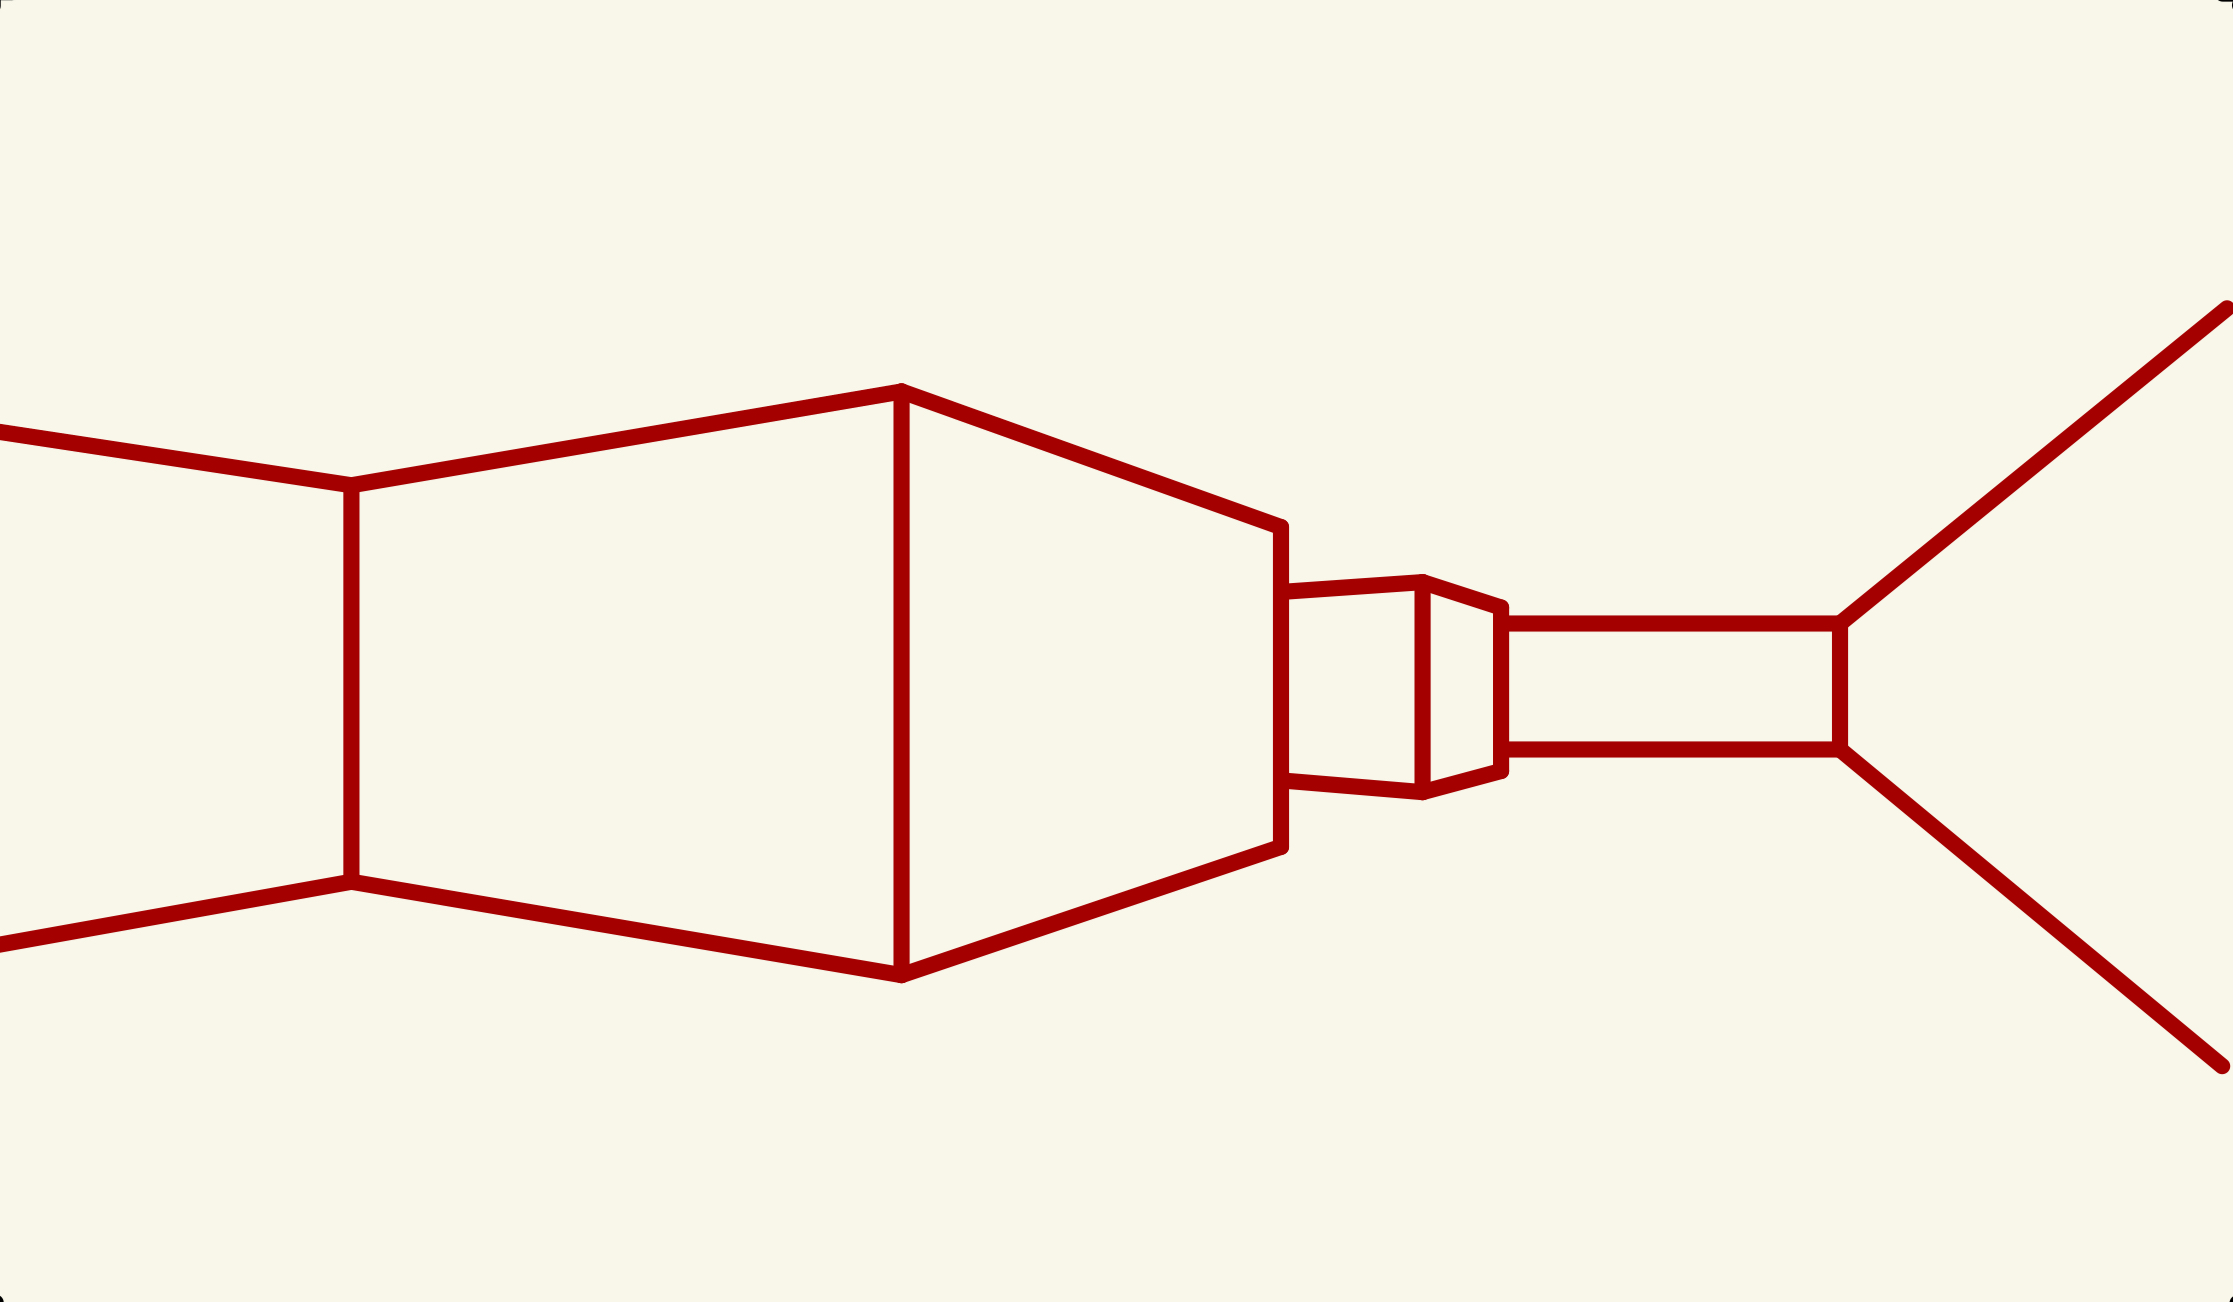
\includegraphics[width=0.7\textwidth]{images/rendu-sans-texture.jpeg}
    \end{figure}
\end{frame}

\begin{frame}
    \frametitle{Les rendus}
    \begin{block}{}
        \begin{itemize}
            \item Résultat avec textures.
        \end{itemize}
    \end{block}
    \begin{figure}
        \centering
        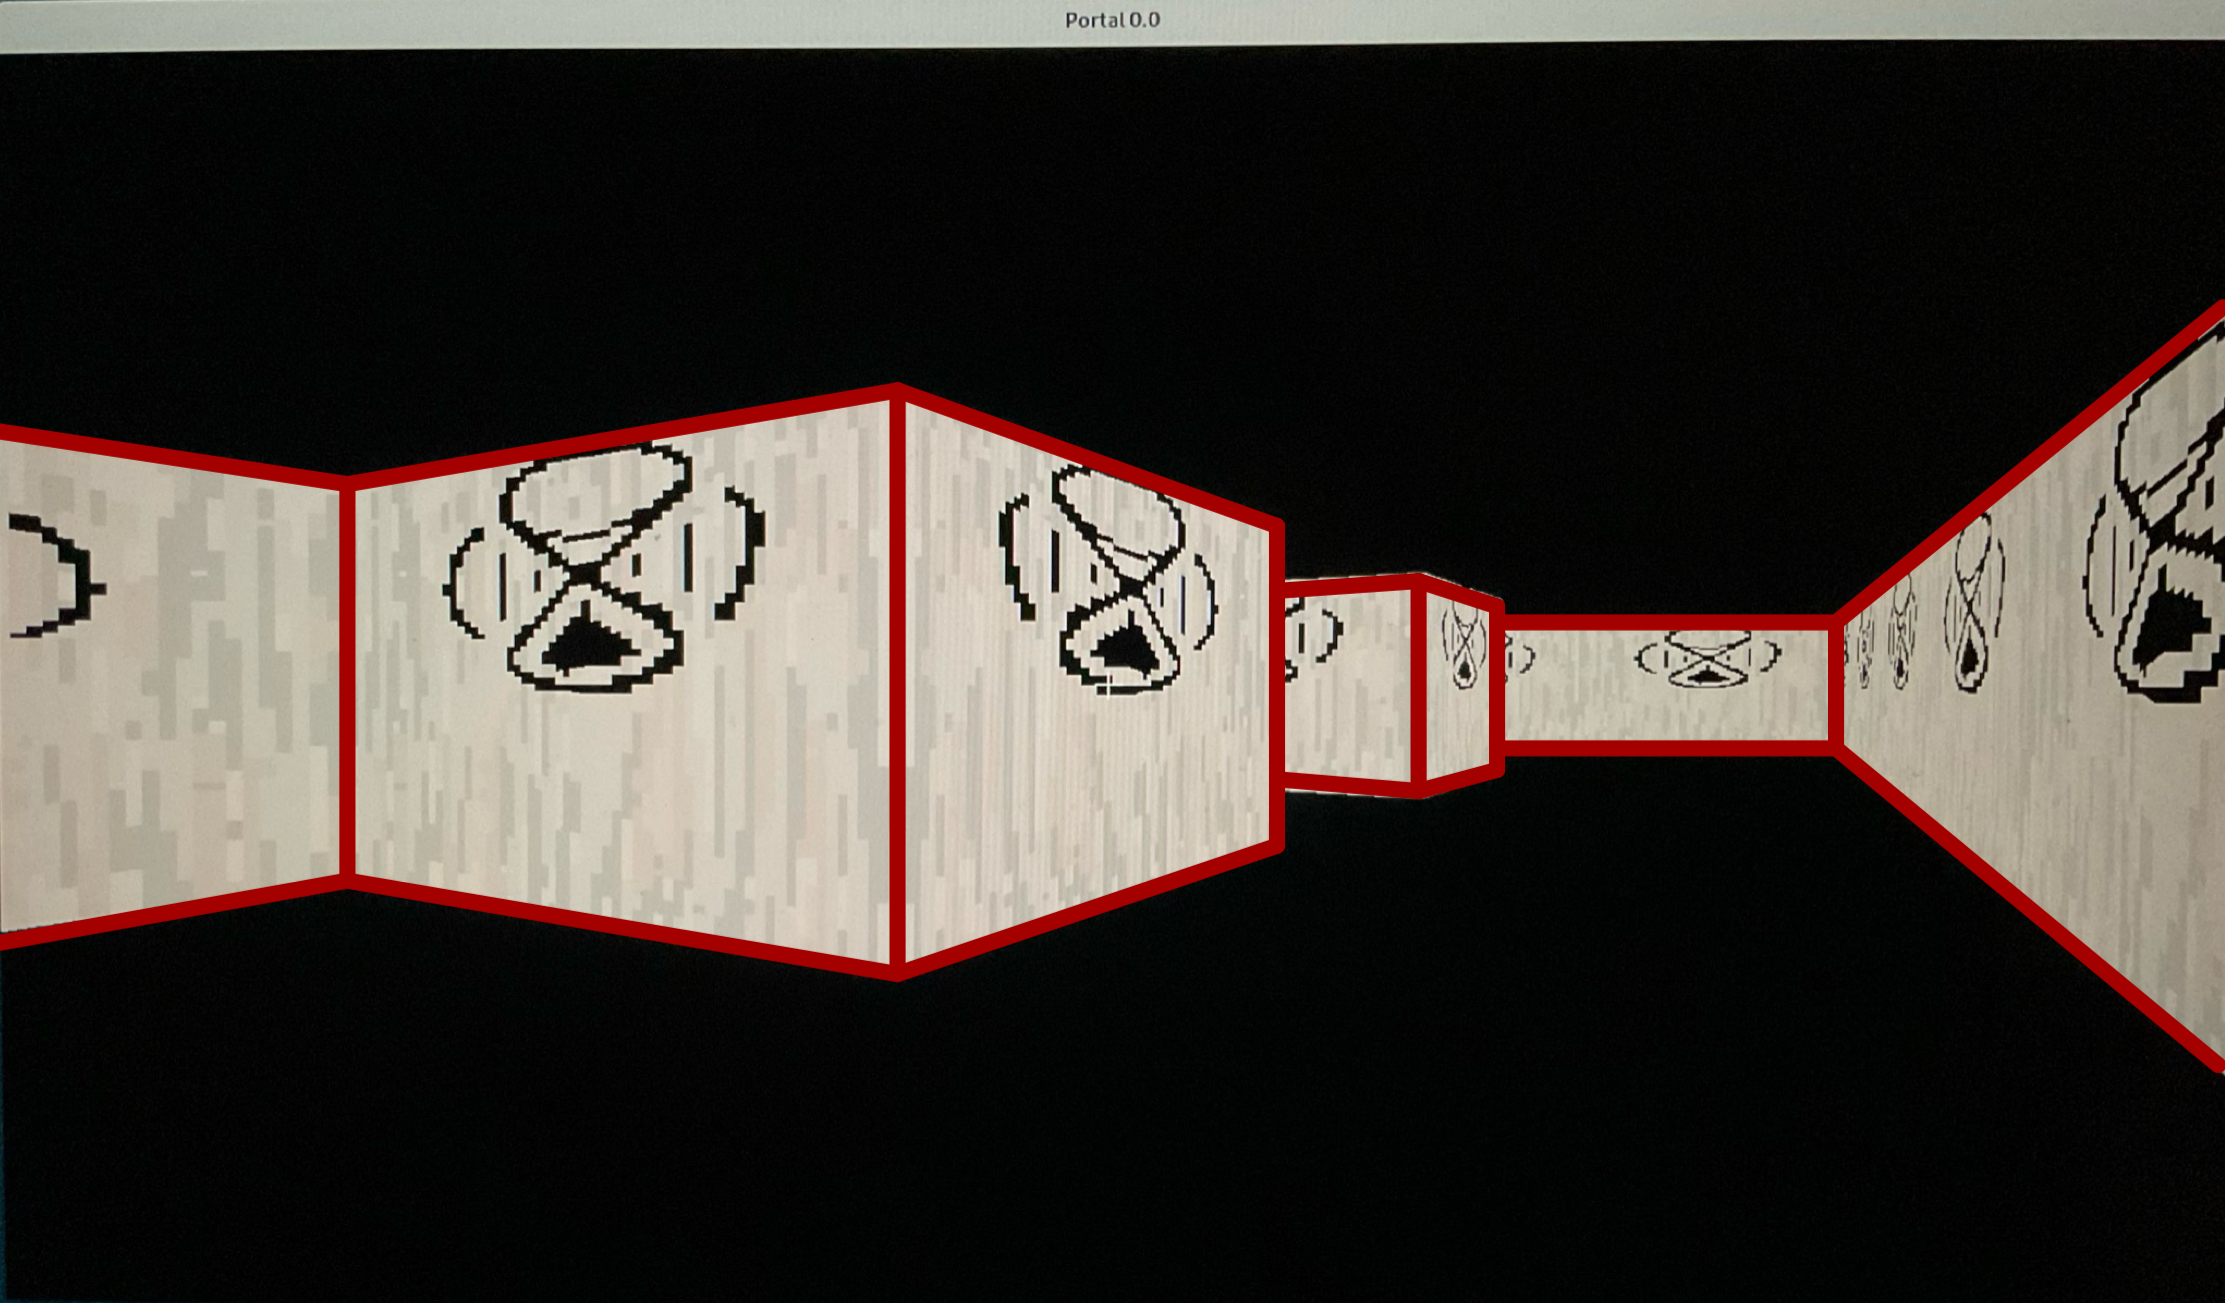
\includegraphics[width=0.7\textwidth]{images/rendu-avec-texture.jpeg}
    \end{figure}
\end{frame}

\subsection{Les portails}

\begin{frame}
    \frametitle{Les portails \\
                \small La téléportation}
    \begin{figure}
        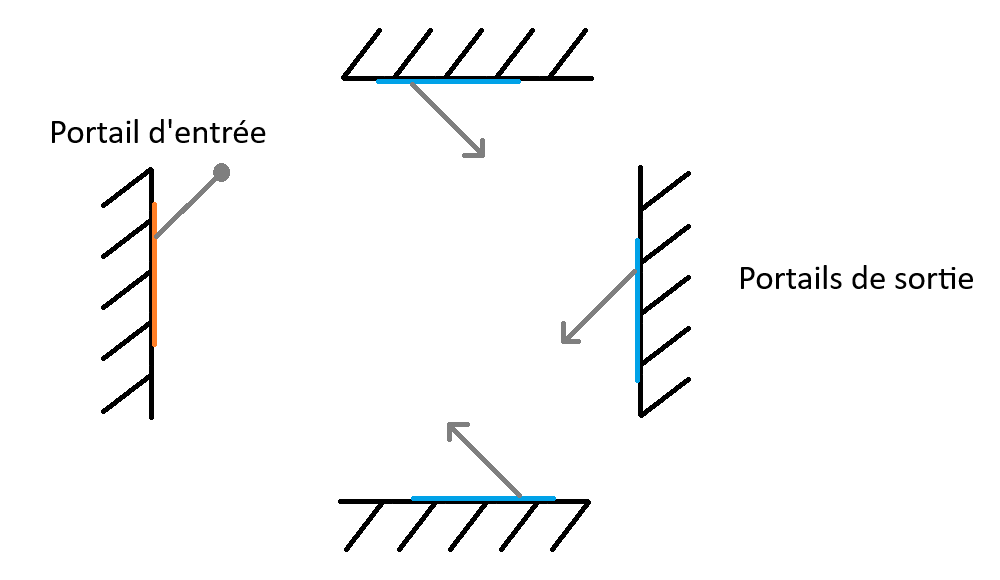
\includegraphics[width=0.5\textwidth]{images/portal2.png}
		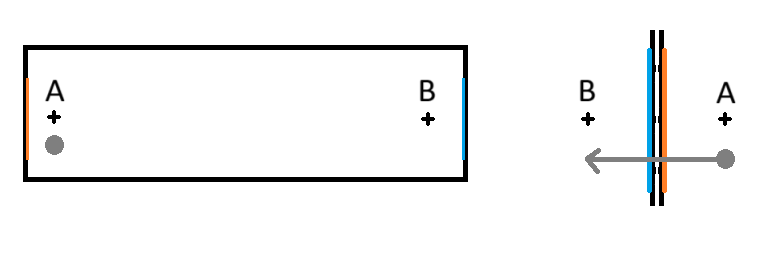
\includegraphics[width=0.45\textwidth]{images/portal3.png}
	\end{figure}
    \begin{block}{}
        \begin{itemize}
            \item Utilisation des cliques gauche et droit
            \item Gain de distance
        \end{itemize}
    \end{block}
    \begin{block}{}
        \begin{itemize}
            \item Réutilisation du système de collision
            \item Rencontre avec un portail
            \begin{itemize}
                \item Calcul du nouvelle angle
                \item Calcul de la nouvelle position
            \end{itemize}
        \end{itemize}
    \end{block}
\end{frame}

\section{Conclusion}

\begin{frame}
    \frametitle{Conclusion}
    \begin{block}{}
        \centering
        Merci de votre attention.
    \end{block}
\end{frame}

\section*{Questions}

\begin{frame}
    \frametitle{Questions}
    \begin{block}{}
        \centering
        Avez-vous des questions ?
    \end{block}
\end{frame}

\end{document}
